\documentclass[]{book}
\usepackage{lmodern}
\usepackage{amssymb,amsmath}
\usepackage{ifxetex,ifluatex}
\usepackage{fixltx2e} % provides \textsubscript
\ifnum 0\ifxetex 1\fi\ifluatex 1\fi=0 % if pdftex
  \usepackage[T1]{fontenc}
  \usepackage[utf8]{inputenc}
\else % if luatex or xelatex
  \ifxetex
    \usepackage{mathspec}
  \else
    \usepackage{fontspec}
  \fi
  \defaultfontfeatures{Ligatures=TeX,Scale=MatchLowercase}
\fi
% use upquote if available, for straight quotes in verbatim environments
\IfFileExists{upquote.sty}{\usepackage{upquote}}{}
% use microtype if available
\IfFileExists{microtype.sty}{%
\usepackage{microtype}
\UseMicrotypeSet[protrusion]{basicmath} % disable protrusion for tt fonts
}{}
\usepackage[margin=1in]{geometry}
\usepackage{hyperref}
\hypersetup{unicode=true,
            pdftitle={Linear Inequalities and Linear Programming},
            pdfauthor={Kevin Cheung},
            pdfborder={0 0 0},
            breaklinks=true}
\urlstyle{same}  % don't use monospace font for urls
\usepackage{natbib}
\bibliographystyle{apalike}
\usepackage{longtable,booktabs}
\usepackage{graphicx,grffile}
\makeatletter
\def\maxwidth{\ifdim\Gin@nat@width>\linewidth\linewidth\else\Gin@nat@width\fi}
\def\maxheight{\ifdim\Gin@nat@height>\textheight\textheight\else\Gin@nat@height\fi}
\makeatother
% Scale images if necessary, so that they will not overflow the page
% margins by default, and it is still possible to overwrite the defaults
% using explicit options in \includegraphics[width, height, ...]{}
\setkeys{Gin}{width=\maxwidth,height=\maxheight,keepaspectratio}
\IfFileExists{parskip.sty}{%
\usepackage{parskip}
}{% else
\setlength{\parindent}{0pt}
\setlength{\parskip}{6pt plus 2pt minus 1pt}
}
\setlength{\emergencystretch}{3em}  % prevent overfull lines
\providecommand{\tightlist}{%
  \setlength{\itemsep}{0pt}\setlength{\parskip}{0pt}}
\setcounter{secnumdepth}{5}
% Redefines (sub)paragraphs to behave more like sections
\ifx\paragraph\undefined\else
\let\oldparagraph\paragraph
\renewcommand{\paragraph}[1]{\oldparagraph{#1}\mbox{}}
\fi
\ifx\subparagraph\undefined\else
\let\oldsubparagraph\subparagraph
\renewcommand{\subparagraph}[1]{\oldsubparagraph{#1}\mbox{}}
\fi

%%% Use protect on footnotes to avoid problems with footnotes in titles
\let\rmarkdownfootnote\footnote%
\def\footnote{\protect\rmarkdownfootnote}

%%% Change title format to be more compact
\usepackage{titling}

% Create subtitle command for use in maketitle
\newcommand{\subtitle}[1]{
  \posttitle{
    \begin{center}\large#1\end{center}
    }
}

\setlength{\droptitle}{-2em}
  \title{Linear Inequalities and Linear Programming}
  \pretitle{\vspace{\droptitle}\centering\huge}
  \posttitle{\par}
  \author{Kevin Cheung}
  \preauthor{\centering\large\emph}
  \postauthor{\par}
  \predate{\centering\large\emph}
  \postdate{\par}
  \date{2017-06-06}

\usepackage{booktabs}
\makeatletter
\def\thm@space@setup{%
  \thm@preskip=8pt plus 2pt minus 4pt
  \thm@postskip=\thm@preskip
}
\makeatother

\def\lt{<}
\def\gt{>}
\newcommand{\NN}{\mathbb{N}}
\newcommand{\ZZ}{\mathbb{Z}}
\newcommand{\QQ}{\mathbb{Q}}
\newcommand{\RR}{\mathbb{R}}
\newcommand{\ssep}{~:~}
\newcommand{\T}{\mathsf{T}}

\newcommand{\mm}[1]{\mathbf{#1}}

\renewcommand{\vec}[1]{\mathbf{#1}}

\renewcommand{\familydefault}{\sfdefault}
\renewcommand{\baselinestretch}{1.2}

\usepackage{amsthm}
\newtheorem{theorem}{Theorem}[chapter]
\newtheorem{lemma}{Lemma}[chapter]
\theoremstyle{definition}
\newtheorem{definition}{Definition}[chapter]
\newtheorem{corollary}{Corollary}[chapter]
\newtheorem{proposition}{Proposition}[chapter]
\theoremstyle{definition}
\newtheorem{example}{Example}[chapter]
\theoremstyle{remark}
\newtheorem*{remark}{Remark}
\let\BeginKnitrBlock\begin \let\EndKnitrBlock\end
\begin{document}
\maketitle

{
\setcounter{tocdepth}{1}
\tableofcontents
}
\renewcommand{\NN}{\mathbb{N}}
\renewcommand{\ZZ}{\mathbb{Z}}
\renewcommand{\QQ}{\mathbb{Q}}
\renewcommand{\RR}{\mathbb{R}}
\renewcommand{\ssep}{~:~}
\renewcommand{\T}{\mathsf{T}}
\renewcommand{\qed}{\square}

\renewcommand{\mm}[1]{\mathbf{#1}}

\renewcommand{\vec}[1]{\mathbf{#1}}

\chapter*{Preface}\label{preface}
\addcontentsline{toc}{chapter}{Preface}

This book covers the fundamentals of linear programming through studying
systems of linear inequalities using only basic facts from linear
algebra. It is suitable for a crash course on linear programming that
emphasizes theoretical aspects of the subject. Discussion on practical
solution methods such as the simplex method and interior point methods,
though not present in this book, is planned for a future book.

Two excellent references for further study are \citet{Bertsimas:1997}
and \citet{Schrijver:1986}.


\includegraphics{images/by-sa.png} The book is licensed under the
\href{http://creativecommons.org/licenses/by-sa/4.0/}{Creative Commons
Attribution-ShareAlike 4.0 International License}.

\chapter*{Notation}\label{notation}
\addcontentsline{toc}{chapter}{Notation}

The set of real numbers is denoted by \(\RR\). The set of rational
numbers is denoted by \(\QQ\). The set of integers is denoted by
\(\ZZ\).

The set of \(n\)-tuples with real entries is denoted by \(\RR^n\).
Similar definitions hold for \(\QQ^n\) and \(\ZZ^n\).

The set of \(m\times n\) matrices (that is, matrices with \(m\) rows and
\(n\) columns) with real entries is denoted \(\RR^{m \times n}\).
Similar definitions hold for \(\QQ^{m\times n}\) and \(\ZZ^n\).

All \(n\)-tuples are written as columns (that is, as \(n\times 1\)
matrices). An \(n\)-tuple is normally represented by a lowercase Roman
letter in boldface; for example, \(\vec{x}\). For an \(n\)-tuple
\(\vec{x}\), \(x_i\) denotes the \(i\)th entry (or component) of
\(\vec{x}\) for \(i = 1,\ldots, n\).

Matrices are normally represented by an uppercase Roman letter in
boldface; for example, \(\mm{A}\). The \(j\)th column of a matrix
\(\mm{A}\) is denoted by \(A_j\) and the \((i,j)\)-entry (that is, the
entry in row \(i\) and column \(j\)) is denoted by \(a_{ij}\).

Scalars are usually represented by lowercase Greek letters; for example,
\(\lambda\), \(\alpha\), \(\beta\) etc.

An \(n\)-tuple consisting of all zeros is denoted by \(\vec{0}\). The
dimension of the tuple is inferred from the context.

For a matrix \(\mm{A}\), \(\mm{A}^\mathsf{T}\) denotes the transpose of
\(\mathbf{A}\). For an \(n\)-tuple \(\mathbf{x}\),
\(\mathbf{x}^\mathsf{T}\) denotes the transpose of \(\mathbf{x}\).

If \(\mm{A}\) and \(\mm{B}\) are \(m\times n\) matrices,
\(\mm{A} \geq \mm{B}\) means \(a_{ij} \geq b_{ij}\) for all
\(i = 1,\ldots, m\), \(j = 1,\ldots, n\). Similar definitions hold for
\(\mm{A} \leq \mm{B}\), \(\mm{A} = \mm{B}\), \(\mm{A} \lt \mm{B}\) and
\(\mm{A} \gt \mm{B}\). In particular, if \(\vec{u}\) and \(\vec{v}\) are
\(n\)-tuples, \(\vec{u}\geq \vec{v}\) means \(u_i \geq v_i\) for
\(i= 1,\ldots, n\) and \(\vec{u} \gt \vec{0}\) means \(u_i \gt 0\) for
\(i = 1,\ldots,n\).

Superscripts in brackets are used for indexing tuples. For example, we
can write \(\vec{u}^{(1)},\vec{u}^{(2)} \in \RR^3\). Then
\(\vec{u}^{(1)}\) and \(\vec{u}^{(2)}\) are elements of \(\RR^3\). The
second entry of \(\vec{u}^{(1)}\) is denoted by \(u^{(1)}_2.\)

\chapter{Graphical example}\label{graphic}

To motivate the subject of linear programming (LP), we begin with a
planning problem that can be solved graphically.

Say you are a vendor of lemonade and lemon juice. Each unit of lemonade
requires 1 lemon and 2 litres of water. Each unit of lemon juice
requires 3 lemons and 1 litre of water. Each unit of lemonade gives a
profit of three dollars. Each unit of lemon juice gives a profit of two
dollars. You have 6 lemons and 4 litres of water available. How many
units of lemonade and lemon juice should you make to maximize profit?

If we let \(x\) denote the number of units of lemonade to be made and
let \(y\) denote the number of units of lemon juice to be made, then the
profit is given by \(3x + 2y\) dollars. We call \(3x + 2y\) the
objective function. Note that there are a number of constraints that
\(x\) and \(y\) must satisfied. First of all, \(x\) and \(y\) should be
nonnegative. The number of lemons needed to make \(x\) units of lemonade
and \(y\) units of lemon juice is \(x+3y\) and cannot exceed 6. The
number of litres of water needed to make \(x\) units of lemonade and
\(y\) units of lemon juice is \(2x+y\) and cannot exceed 4. Hence, to
determine the maximum profit, we need to maximize \(3x + 2y\) subject to
\(x\) and \(y\) satisfying the constraints \(x + 3y \leq 6\),
\(2x + y \leq 4\), \(x \geq 0\), and \(y \geq 0.\)

A more compact way to write the problem is as follows:
\[\begin{array}{rrcrll}
\mbox{maximize } & 3x & + & 2y & \\
\mbox{subject to} 
& x & + & 3y & \leq & 6 \\
& 2x & +&  y & \leq & 4 \\
& x &  & & \geq & 0 \\
& & & y & \geq & 0. \\
\end{array}\]

We can solve this maximizationproblem graphically as follows. We first
sketch the set of \(\begin{bmatrix} x\\ y\end{bmatrix}\) satisfying the
constraints, called the feasible region, on the \((x,y)\)-plane. We then
take the objective function \(3x+2y\) and turn it into an equation of a
line \(3x+2y = z\) where \(z\) is a parameter. Note that as the value of
\(z\) increases, the line defined by the equation \(3x+2y=z\) moves in
the direction of the normal vector
\(\begin{bmatrix} 3 \\ 2\end{bmatrix}\). We call this direction the
direction of improvement. Determining the maximum value of the objective
function, called the optimal value, subject to the contraints amounts to
finding the maximum value of \(z\) so that the line defined by the
equation \(3x+2y=z\) still intersects the feasible region.

\begin{center}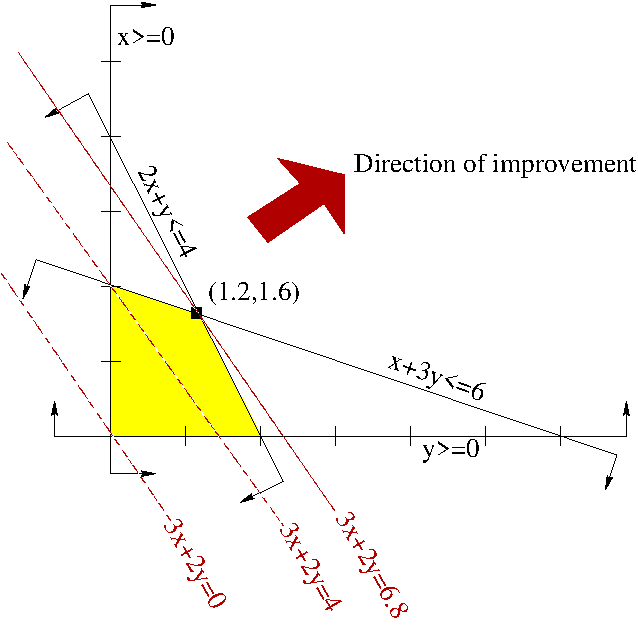
\includegraphics[width=0.8\linewidth]{images/lemon} \end{center}

In the figure above, the lines with \(z\) at 0, 4 and 6.8 have been
drawn. From the picture, we can see that if \(z\) is greater than 6.8,
the line defined by \(3x+2y = z\) will not intersect the feasible
region. Hence, the profit cannot exceed 6.8 dollars.

As the line \(3x+2y = 6.8\) does intersect the feasible region, \(6.8\)
is the maximum value for the objective function. Note that there is only
one point in the feasible region that intersects the line \(3x+2y=6.8\),
namely
\(\begin{bmatrix} x \\ y\end{bmatrix} = \begin{bmatrix} 1.2 \\ 1.6\end{bmatrix}.\)
In other words, to maximize profit, we want to make 1.2 units of
lemonade and 1.6 units of lemon juice.

The above solution method can hardly be regarded as rigorous because we
relied on a picture to conclude that \(3x + 2y \leq 6.8\) for all
\(\begin{bmatrix} x\\y\end{bmatrix}\) satisfying the constraints. But we
can actually show this \emph{algebraically}.

Note that multiplying both sides of the constraint \(x + 3y \leq 6\)
gives \(0.2x + 0.6 y \leq 1.2\), and multiplying both sides of the
constraint \(2x + y \leq 4\) gives \(2.8x + 1.4 y \leq 5.6\). Hence, any
\(\begin{bmatrix} x\\y\end{bmatrix}\) that satisfies both \(x+3y\leq 6\)
and \(2x+y \leq 4\) must also satisfy
\((0.2x+0.6y) + (2.8x+1.4y) \leq 1.2 + 5.6\), which simplifies to
\(3x + 2y \leq 6.8\) as desired! (Here, we used the fact that if
\(a \leq b\) and \(c \leq d\), then \(a+c \leq b+d\).)

Now, one might ask if it is always possible to find an algebraic proof
like the one above for similar problems. If the answer is yes, how does
one find such a proof? We will see answers to this question later on.

Before we end this segment, let us consider the following problem:
\[\begin{array}{rrcrll}
\mbox{minimize } & -2x & + & y & \\
\mbox{subject to} & -x & + & y & \leq & 3 \\
& x & - &  2y & \leq & 2 \\
& x &  & & \geq & 0 \\
& & & y & \geq & 0. \\
\end{array}\]

Note that for any \(t \geq 0\),
\(\begin{bmatrix} x \\ y\end{bmatrix} = \begin{bmatrix} t \\ t\end{bmatrix}\)
satisfies all the constraints. The value of the objective function at
\(\begin{bmatrix} x \\ y\end{bmatrix} = \begin{bmatrix} t \\ t\end{bmatrix}\)
is \(-t\). As \(t \rightarrow \infty\), the value of the objective
function tends to \(-\infty\). Therefore, there is no minimum value for
the objective function. The problem is said to be unbounded. Later on,
we will see how to detect unboundedness algorithmically.

As an exercise, check that unboundedness can also be established by
using
\(\begin{bmatrix} x \\ y\end{bmatrix} = \begin{bmatrix} 2t+2 \\ t\end{bmatrix}\)
for \(t \geq 0\).

\section*{Exercises}\label{exercises}
\addcontentsline{toc}{section}{Exercises}

\begin{enumerate}
\def\labelenumi{\arabic{enumi}.}
\item
  Sketch all \(\begin{bmatrix} x \\ y \end{bmatrix}\) satisfying

  \begin{equation*}
  x - 2y \leq 2
  \end{equation*}

  on the \((x,y)\)-plane.
\item
  Determine the optimal value of \[
  \begin{array}{rl}
  \text{Minimize} & x + y \\
  \text{Subject to} &  2x + y \geq 4 \\
  & x + 3y \geq 1.
  \end{array}
  \]
\item
  Show that the problem \[
  \begin{array}{rl}
  \text{Minimize} & -x + y \\
  \text{Subject to} &  2x - y \geq 0 \\
  & x + 3y \geq 3
  \end{array}
  \] is unbounded.
\item
  Suppose that you are shopping for dietary supplements to satisfy your
  required daily intake of 0.40mg of nutrient \(M\) and 0.30mg of
  nutrient \(N\). There are three popular products on the market. The
  costs and the amounts of the two nutrients are given in the following
  table:

  \begin{longtable}[]{@{}lccc@{}}
  \toprule
  & Product 1 & Product 2 & Product 3\tabularnewline
  \midrule
  \endhead
  Cost & \$27 & \$31 & \$24\tabularnewline
  Daily amount of \(M\) & 0.16 mg & 0.21 mg & 0.11 mg\tabularnewline
  Daily amount of \(N\) & 0.19 mg & 0.13 mg & 0.15 mg\tabularnewline
  \bottomrule
  \end{longtable}

  You want to determine how much of each product you should buy so that
  the daily intake requirements of the two nutrients are satisfied at
  minimum cost. Formulate your problem as a linear programming problem,
  assuming that you can buy a fractional number of each product.
\end{enumerate}

\section*{Solutions}\label{solutions}
\addcontentsline{toc}{section}{Solutions}

\begin{enumerate}
\def\labelenumi{\arabic{enumi}.}
\item
  The points \((x,y)\) satisfying \(x-2y \leq 2\) are precisely those
  above the line passing through \((2,0)\) and \((0,-1)\).
\item
  We want to determine the minimum value \(z\) so that \(x+y=z\) defines
  a line that has a nonempty intersection with the feasible region.
  However, we can avoid referring to a sketch by setting \(x=z-y\) and
  substituting for \(x\) in the inequalities to obtain:

  \begin{eqnarray*}
   2(z-y) + y \geq 4 \\
   (z-y) + 3y \geq 1,
  \end{eqnarray*}

  or equivalently,

  \begin{eqnarray*}
   z \geq 2+\frac{1}{2}y \\
   z \geq 1-2y,
  \end{eqnarray*}

  Thus, the minimum value for \(z\) is
  \(\min \{ 2+\frac{1}{2}y, 1-2y\}\), which occurs at
  \(y = -\frac{2}{5}\). Hence, the optimal value is \(\frac{9}{5}\).

  We can verify our work by doing the following. If our calculations
  above are correct, then an optimal solution is given by
  \(x = \frac{11}{5}\), \(y = -\frac{2}{5}\) since \(x = z - y\). It is
  easy to check that this satisfies both inequalities and therefore is a
  feasible solution.

  Now, taking \(\frac{2}{5}\) times the first inequality and
  \(\frac{1}{5}\) times the second inequality, we can infer the
  inequality \(x+y \geq \frac{9}{5}\). The left-hand side of this
  inequality is precisely the objective function. Hence, no feasible
  solution can have objective function value less than \(\frac{9}{5}\).
  But \(x = \frac{11}{5}\), \(y = -\frac{2}{5}\) is a feasible solution
  with objective function value equal to \(\frac{9}{5}\). As a result,
  it must be an optimal solution.

  \textbf{Remark.} We have not yet discussed how to obtain the
  multipliers \(\frac{2}{5}\) and \(\frac{1}{5}\) for inferring the
  inequality \(x+y \geq \frac{9}{5}\). This is an issue that will be
  taken up later. In the meantime, think about how one could have
  obtained these multipliers for this particular exercise.
\item
  We could glean some insight by first making a sketch on the
  \((x,y)\)-plane.

  The line defined by \(-x + y = z\) has \(x\)-intercept \(-z\). Note
  that for \(z \leq -3\),
  \(\begin{bmatrix} x\\y \end{bmatrix} = \begin{bmatrix} -z\\ 0\end{bmatrix}\)
  satisfies both inequalities and the value of the objective function at
  \(\begin{bmatrix} x\\y \end{bmatrix} = \begin{bmatrix} -z\\ 0\end{bmatrix}\)
  is \(z\). Hence, there is no lower bound on the value of objective
  function.
\item
  Let \(x_i\) denote the amount of Product \(i\) to buy for
  \(i = 1,2,3\). Then, the problem can be formulated as
  \[\begin{array}{rrcrcrll}
  \mbox{minimize } & 27 x_1 & + & 31 x_2 & + & 24 x_3 \\
  \mbox{subject to} 
  & 0.16 x_1 & + & 0.21 x_2 & + & 0.11 x_3 & \geq & 0.30 \\
  & 0.19 x_1 & + & 0.13 x_2 & + & 0.15 x_3 & \geq & 0.40 \\
  & x_1 & , & x_2 & , & x_3 & \geq & 0. \\
  \end{array}\]

  \textbf{Remark.} If one cannot buy fractional amounts of the products,
  the problem can be formulated as \[\begin{array}{rrcrcrll}
  \mbox{minimize } & 27 x_1 & + & 31 x_2 & + & 24 x_3 \\
  \mbox{subject to} 
  & 0.16 x_1 & + & 0.21 x_2 & + & 0.11 x_3 & \geq & 0.30 \\
  & 0.19 x_1 & + & 0.13 x_2 & + & 0.15 x_3 & \geq & 0.40 \\
  & x_1 & , & x_2 & , & x_3 & \geq & 0. \\
  & x_1 & , & x_2 & , & x_3 & \in & \mathbb{Z}. \\
  \end{array}\]
\end{enumerate}

\chapter{Definitions}\label{definitions}

The following is an example of a problem in \textbf{linear programming}:
\[
\begin{array}{rl}
\text{Maximize} & x + y - 2z \\
\text{Subject to} &  2x + y + z \leq 4 \\
& 3x - y + z = 0 \\
&  x, y, z \geq 0
\end{array}
\] \textbf{Solving} this problem means finding real values for the
\textbf{variables} \(x,y,z\) satisfying the \textbf{constraints}
\(2x + y + z \leq 4\), \(3x-y +z =0\), and \(x,y,z \geq 0\) that gives
the maximum possible value (if it exists) for the \textbf{objective
function} \(x + y - 2z\).

For example,
\(\begin{bmatrix} x\\y\\z\end{bmatrix} = \begin{bmatrix} 0 \\ 1 \\ 1\end{bmatrix}\)
satisfies all the constraints and is called a \textbf{feasible
solution}. Its \textbf{objective function value}, obtained by evaluating
the objective function at
\(\begin{bmatrix} x\\y\\z\end{bmatrix} = \begin{bmatrix} 0 \\ 1 \\ 1\end{bmatrix}\),
is \(0 + 1 - 2(1) = -1\). The set of feasible solutions to a linear
programming problem is called the \textbf{feasible region}.

More formally, a linear programming problem is an optimization problem
of the following form: \[
\begin{array}{rll}
\text{Maximize (or Minimize)} & \displaystyle\sum_{j=1}^n c_j x_j \\
\text{Subject to} &  P_i(x_1, \ldots, x_n) & i = 1,\ldots, m
\end{array}
\] where \(m\) and \(n\) are positive integers, \(c_j \in \RR\) for
\(j = 1,\ldots, n\), and for each \(i = 1,\ldots, m\),
\(P_i(x_1,\ldots, x_n)\) is a \textbf{linear constraint} on the
\textbf{(decision) variables} \(x_1,\ldots, x_n\) having one of the
following forms:

\begin{itemize}
\tightlist
\item
  \(a_1 x_1 + \cdots + a_n x_n \geq \beta\)
\item
  \(a_1 x_1 + \cdots + a_n x_n \leq \beta\)
\item
  \(a_1 x_1 + \cdots a_n x_n = \beta\)
\end{itemize}

where \(\beta, a_1,\ldots, a_n \in \RR\). To save writing, the word
``Minimize'' (``Maximize'') is replaced with ``\(\min\)'' (``\(\max\)'')
and ``Subject to'' is abbreviated as ``\(\text{s.t.}\)''.

A feasible solution
\(\vec{x} = \begin{bmatrix} x_1 \\ \vdots \\ x_n\end{bmatrix}\) that
gives the maximum possible objective function value in the case of a
maximization problem is called an \textbf{optimal solution} and its
objective function value is the \textbf{optimal value} of the problem.

The following example shows that it is possible to have multiple optimal
solutions: \[
\begin{array}{rl}
\max & x + y\\
\text{s.t.} &  2x + 2y\leq 1
\end{array}
\] The constraint says that \(x+y\) cannot exceed \(\frac{1}{2}\). Now,
both
\(\begin{bmatrix}x\\y\end{bmatrix} = \begin{bmatrix}\frac{1}{2}\\ 0\end{bmatrix}\)
and
\(\begin{bmatrix}x\\y\end{bmatrix} = \begin{bmatrix}0\\\frac{1}{2}\end{bmatrix}\)
are feasible solutions having objective function value \(\frac{1}{2}\).
Hence, they are both optimal solutions. (In fact, this problem has
infinitely many optimal solutions. Can you specify all of them?)

Not all linear programming problems have optimal solutions. For example,
a problem can have no feasible solution. Such a problem is said to be
\textbf{infeasible}. Here is an example of an infeasible problem: \[
\begin{array}{rl}
\min & x \\
\text{s.t.} &  x \leq 1 \\
& x \geq 2
\end{array}
\] There is no value for \(x\) that is at the same time at most 1 and at
least 2.

Even if a problem is not infeasible, it might not have an optimal
solution as the following example shows: \[
\begin{array}{rl}
\min & x \\
\text{s.t.} &  x \leq 0
\end{array}
\] Note that now matter what real number \(M\) we are given, we can
always find a feasible solution whose objective function value is less
than \(M\). Such a problem is said to be \textbf{unbounded}. (For a
maximization problem, it is unbounded if one can find feasible solutions
who objective function value is larger than any given real number.)

\begin{center}\rule{0.5\linewidth}{\linethickness}\end{center}

So far, we have seen that a linear programming problem can have an
optimal solution, be infeasible, or be unbounded. Is it possible for a
linear programming problem to be not infeasible, not unbounded, and with
no optimal solution?\\
The following optimization problem, though not a linear programming
problem, is not infeasible, not unbounded, and has no optimal solution:
\[
\begin{array}{rl}
\min & 2^x \\
\text{s.t.} &  x \leq 0
\end{array}
\] The objective function value is never negative and can get
arbitrarily close to 0 but can never attain 0.

A main result in linear programming states that if a linear programming
problem is not infeasible and is not unbounded, then it must have an
optimal solution. This result is known as the \textbf{Fundamental
Theorem of Linear Programming} (Theorem \ref{thm:fund-lp}) and we will
see a proof of this importan result. In the meantime, we will consider
the seemingly easier problem of determining if a system of linear
constraints has a solution.

\section*{Exercises}\label{exercises-1}
\addcontentsline{toc}{section}{Exercises}

\begin{enumerate}
\def\labelenumi{\arabic{enumi}.}
\item
  Determine all values of \(a\) such that the problem \[
  \begin{array}{rl}
  \min & x + y \\
  \text{s.t.} 
  &  -3x + y \geq a \\
  &  2x - y \geq 0 \\
  & x + 2y \geq 2
  \end{array}
  \] is infeasible.
\item
  Show that the problem \[
  \begin{array}{rl}
  \min & 2^x \cdot 4^y \\
  \text{s.t.} 
  &  e^{-3x + y} \geq 1 \\
  &  |2x - y| \leq 4 \\
  \end{array}
  \] can be solved by solving a linear programming problem.
\end{enumerate}

\section*{Solutions}\label{solutions-1}
\addcontentsline{toc}{section}{Solutions}

\begin{enumerate}
\def\labelenumi{\arabic{enumi}.}
\item
  Adding the first two inequalities gives \(-x \geq a\). Adding \(2\)
  times the second inequality and the third inequality gives
  \(5x \geq 2\), implying that \(x \geq \frac{2}{5}\). Hence, if
  \(a \gt -\frac{2}{5}\), there is no solution.

  Note that if \(a \leq -\frac{2}{5}\), then
  \((x,y) = \left (\frac{2}{5}, \frac{4}{5}\right)\) satisfies all the
  inequalities. Hence, the problem is infeasible if and only if
  \(a \gt -\frac{2}{5}\).
\item
  Note that the constraint \(|2x - y| \leq 4\) is equivalent to the
  constraints \(2x-y\leq 4\) and \(2x-y \geq -4\) taken together, and
  the constraint \(e^{-3x+y} \geq 1\) is equivalent to \(-3x+y \geq 0\).
  Hence, we can rewrite the problem with linear constraints.

  Finally, minimizing \(2^x \cdot 4^y\) is the same as minimizing
  \(2^{x + 2y}\), which is equivalent to minimizing \(x+2y\).
\end{enumerate}

\chapter{Inferring linear
constraints}\label{inferring-linear-constraints}

If \(a\), \(b\), \(c\), and \(d\) are real numbers such that
\(a \geq b\) and \(c \geq d\), then \(a + c \geq b + d\). We say that
\(a + c \geq b + d\) is \textbf{inferred} from \(a \geq b\) and
\(c \geq d\). Casually, we also say that ``adding'' the two inequalities
gives \(a + c \geq b + d\).

Note that adding inequalities require that the inequalities to have the
same sense; in other words, adding a mixture of \(\leq\)-inequalities
and \(\geq\)-inequalities is not allowed for obvious reason. However,
adding a mixture of inequalities having the same sense and equations is
valid. For example, if \(x\) and \(y\) are real numbers satisfying
\begin{align*}
x - 2y & \geq 5 \\
3x + y & = 7,
\end{align*}

then \(x\) and \(y\) must also satisfy \(4x - y \geq 12\).

Going one step further, we can add scalar multiples of inequalities to
obtain new inequalities under appropriate conditions. For example, if
\(a\geq b\), \(c \leq d\), \(\alpha \geq 0\), and \(\beta \leq 0\), then
\(\alpha a + \beta c \geq \alpha b + \beta d\).

In general, suppose that \(\vec{x} \in \RR^n\) satisfies the system
\begin{align}
\begin{split}
\mm{P} \vec{x} & \geq \vec{p} \\
\mm{Q} \vec{x} & \leq \vec{q} \\
\mm{R} \vec{x} & = \vec{r} 
\end{split}
\label{eq:mixed-sys}
\end{align}

where \(\mm{P} \in \RR^{m \times n}\), \(\vec{p} \in \RR^m\),
\(\mm{Q} \in \RR^{m' \times n}\), \(\vec{q} \in \RR^{m'}\),
\(\mm{R} \in \RR^{\bar{m} \times n}\), \(\vec{r} \in \RR^{\bar{m}}\) for
some nonnegative integers \(m, m', \bar{m}\). If \(\vec{f} \in \RR^m\)
with \(\vec{f} \geq \vec{0}\), \(\vec{g} \in \RR^{m'}\) with
\(\vec{g} \leq \vec{0}\), and \(\vec{h} \in \RR^{\bar{m}}\), then
\(\vec{x}\) also satisfies \[ \vec{c}^\T \vec{x} \geq \gamma\] where
\(\vec{c} =  \vec{f}^\T\mm{P}+ \vec{g}^\T \mm{Q} +\vec{h}^\T \mm{R}\)
and
\(\gamma =  \vec{f}^\T\vec{p}+ \vec{g}^\T \vec{q} +\vec{h}^\T \vec{r}\).
We say that the inequality \(\vec{c}^\T \vec{x} \geq \gamma\) is
\emph{inferred} from the system \eqref{eq:mixed-sys}. To simplify the
language for describing linear constraint inference, we often assign
labels to the constraints and write linear combinations of them. For
example, say we have the system
\begin{align}
x_1 + 2x_2 & \geq 2  \label{eq:lin-comb-geq} \\
-x_1 + x_2 & \leq 1  \label{eq:lin-comb-leq} \\
3x_1 - x_2 & = -1.  \label{eq:lin-comb-eq}
\end{align}

Then \(2\times\) \eqref{eq:lin-comb-geq} \(+\) \((-1)\times\)
\eqref{eq:lin-comb-leq} \(+\) \eqref{eq:lin-comb-eq} refers to the
inequality \(6x_1+2x_2 \geq 2\) since
\(2(x_1+2x_2)+(-1)(-x_1+x_2)+(3x_1 - x_2)\) gives \(6x_1 + 2x_2\) and
\(2(2) + (-1)(1) + (-1)\) is \(2\).

\section*{Exercises}\label{exercises-2}
\addcontentsline{toc}{section}{Exercises}

\begin{enumerate}
\def\labelenumi{\arabic{enumi}.}
\tightlist
\item
  Determine the smallest value of \(\mu\) such that \(x + y \geq \mu\)
  can be inferred from the system
  \begin{align*}
  2x + y & \geq 2 \\
  x + 3y & \geq 1 \\
  3x + 2y & \geq 6
  \end{align*}
\item
  Show that the inequality \(x + 2y \geq 3\) can be inferred from the
  system
  \begin{align*}
  2x + y & \geq 2 \\
  x + 5y & \geq 7 \\
  -x + y & = 1 \\
  \end{align*}

  in infinitely many ways.
\end{enumerate}

\section*{Solutions}\label{solutions-2}
\addcontentsline{toc}{section}{Solutions}

\begin{enumerate}
\def\labelenumi{\arabic{enumi}.}
\tightlist
\item
  To infer \(x + y \geq \mu\) from the given system, we need
  \(\alpha \geq 0\), \(\beta \geq 0\), and \(\gamma \geq 0\) such that
  \begin{align*}
    2\alpha + \beta + 3\gamma & = 1\\
     \alpha + 3\beta + 2\gamma & = 1\\
    2\alpha + \beta + 6\gamma & = \mu.
  \end{align*}

  Solving gives
  \(\begin{bmatrix} \alpha \\ \beta \\ \gamma\end{bmatrix} = \begin{bmatrix} \frac{13}{15} - \frac{7}{15} \mu \\ \frac{4}{15}-\frac{1}{15} \mu \\ -\frac{1}{3} + \frac{1}{3}\mu\end{bmatrix}\).
  The largest value \(\mu\) can take so that this tuple has only
  nonnegative entries is \(\frac{13}{7}\).
\item
  We first label the constraints:
  \begin{align}
  2x + y & \geq 2 \label{eq:inf-ex2-1} \\
  x + 5y & \geq 7 \label{eq:inf-ex2-2} \\
  -x + y & = 1.  \label{eq:inf-ex2-3}
  \end{align}

  Let
  \(C = \left \{ \lambda \begin{bmatrix} 1 \\ 0 \\ 1\end{bmatrix} + (1-\lambda)\begin{bmatrix} \frac{1}{3} \\ \frac{1}{3} \\ 0 \end{bmatrix} \ssep 0 \leq \lambda \leq 1 \right\}\).
  Note that \(C\) has infinitely many elements and that for every
  \(\begin{bmatrix} \alpha \\ \beta \\ \gamma\end{bmatrix} \in C\),
  \(\alpha \times\) \eqref{eq:inf-ex2-1} \(+\) \(\beta \times\)
  \eqref{eq:inf-ex2-2} \(+\) \(\gamma \times\) \eqref{eq:inf-ex2-3} gives
  the constraint \(x + 2y \geq 3\).

  For example, when \(\lambda = \frac{1}{2}\),
  \(\lambda \begin{bmatrix} 1 \\ 0 \\ 1\end{bmatrix} + (1-\lambda)\begin{bmatrix} \frac{1}{3} \\ \frac{1}{3} \\ 0 \end{bmatrix} = \begin{bmatrix} \frac{2}{3} \\ \frac{1}{6} \\ \frac{1}{2}\end{bmatrix}\).
\end{enumerate}

\chapter{Solving systems of linear
inequalities}\label{solving-systems-of-linear-inequalities}

Before we can solve a linear programming problem, we should be able to
solve the seemingly simpler problem of finding a feasible solution. We
will now consider how one can determine if a system of linear
inequalities has a solution.

For the sake of illustrating the principles involved, we limit ourselves
to systems consisting of only \(\geq\)-inequalities. Extending the
method to work with any systems of linear constraints is left as an
exercise.

Suppose that we want to determine if there exist \(x,y\in\mathbb{R}\)
satisfying
\begin{align*}
x + y & \geq 0 \\
2x + y & \geq 2 \\
-x + y  & \geq 1 \\
-x + 2y & \geq -1.
\end{align*}

The key is to take one of the variables and see how it is constrained by
the remaining variables. We ``isolate'' \(x\) by rewriting the system to
the equivalent system
\begin{align*}
x & \geq -y  \\
x & \geq 1 - \frac{1}{2}y \\
x & \leq -1 +y \\
x & \leq 1 + 2y.
\end{align*}

Hence, \(x\) is constrained by the lower bounds \(-y\) and
\(1 - \frac{1}{2}y\) and the upper bounds \(-1 +y\) and \(1 + 2y\).
Therefore, we can find a value for \(x\) satisfying these bounds if and
only if each of the upper bounds is at least each of the lower bounds;
that is,
\begin{align*}
-1 + y & \geq -y \\
-1 + y & \geq 1 - \frac{1}{2}y \\
1 + 2y & \geq -y \\
1 + 2y & \geq 1 - \frac{1}{2}y.
\end{align*}

Simplifying this system gives
\begin{align*}
2y & \geq 1 \\
\frac{3}{2}y & \geq 2  \\
3y & \geq -1 \\
\frac{5}{2}y & \geq 0,
\end{align*}

or more simply,
\begin{align*}
y & \geq \frac{1}{2} \\
y & \geq \frac{4}{3}  \\
y & \geq -\frac{1}{3} \\
y & \geq 0.
\end{align*}

Note that this system does not contain the variable \(x\) and it has a
solution if and only if \(y \geq \frac{4}{3}\). Hence, the original
system has a solution if and only if \(y \geq \frac{4}{3}\). If we set
\(y = 2\), for example, then \(x\) must satisfy
\begin{align*}
x & \geq - 2  \\
x & \geq 0 \\
x & \leq 1 \\
x & \leq 5.
\end{align*}

Thus, we can pick \(x\) to be any value in the closed interval
\([0,1]\). In particular,
\(\begin{bmatrix} x\\ y\end{bmatrix} = \begin{bmatrix} 0 \\ 2\end{bmatrix}\)
is \emph{one} solution to the given system of linear inequalities. There
could be other solutions.

The above example illustrates the process of solving a system of linear
inequaltiies by constructing a system that has a reduced number of
variables. As the number of variables is finite, the process can be
repeated until we obtain a system whose solvability is apparent (as in
the one-variable case).

Observe that the pairing of an upper bound constraint of the form
\(x \leq q\) and a lower bound constraint of the form \(x \geq p\) to
obtain \(q \geq p\) is equivalent to adding the inequalities
\(-x \geq -q\) and \(x \geq p\). This observation leads to the
following:

\hypertarget{fm}{\section{Fourier-Motzkin Elimination}\label{fm}}

Given: A system of linear inequalities
\[ \sum_{j=1}^n a_{ij} x_j \geq b_i,~~~i = 1,\ldots,m\] where
\(a_{ij}, b_i \in \mathbb{R}\) for \(i = 1,\ldots,m\) and
\(j = 1,\ldots,n\),

Eliminate \(x_k\) for some \(k \in \{1,\ldots,n\}\) using the following
steps:

\begin{enumerate}
\def\labelenumi{\arabic{enumi}.}
\item
  For each \(j \in \{1,\ldots m\}\),

  \begin{itemize}
  \tightlist
  \item
    if \(a_{jk} \gt 0\), multiply the \(j\)th inequality by
    \(\frac{1}{a_{jk}}\),
  \item
    if \(a_{jk} \lt 0\), multiply the \(j\)th inequality by
    \(-\frac{1}{a_{jk}}\)
  \end{itemize}
\item
  Form a new system of inequalities as follows:

  \begin{itemize}
  \tightlist
  \item
    copy down all the inequalities in which the coefficient of \(x_k\)
    is 0
  \item
    for each inequality in which \(x_k\) has positive coefficent and for
    each inequality in which \(x_k\) has negative coefficient, obtain a
    new inequality by adding them together.
  \end{itemize}
\end{enumerate}

\textbf{Remarks.}

\begin{enumerate}
\def\labelenumi{\arabic{enumi}.}
\item
  Step 1 is to ensure that all the nonzero coefficients of \(x_k\) are
  \(1\) or \(-1\).
\item
  The new system formed in Step 2 will not contain the variable \(x_k\).
  Furthermore, if \(x_1^*,\ldots, x_n^*\) is a solution to the original
  system, then \(x_1^*,\ldots,x_{k-1}^*, x_{k+1}^*,\ldots, x_n^*\) is a
  solution to the new system. And if
  \(x_1^*,\ldots,x_{k-1}^*, x_{k+1}^*,\ldots, x_n^*\) is a solution to
  the new system, then there exists \(x_k^*\) such that
  \(x_1^*,\ldots, x_n^*\) is a solution to the original system. (Why?)
  Hence, the original system has a solution if and only if the new
  system does.
\end{enumerate}

Now, if we apply Fourier-Motzkin elimination repeatedly, we obtain a
system with at most one variable such that it has a solution if and only
if the original system does. Since solving systems of linear
inequalities with at most one variable is easy, we can conclude whether
or not the original system has a solution.

Note that if the coefficients are all rational, the system obtained
after eliminating one variable using Fourier-Motzkin elimination will
also have only rational coefficients.

\BeginKnitrBlock{example}
\protect\hypertarget{ex:unnamed-chunk-1}{}{\label{ex:unnamed-chunk-1}}Determine
if the following system of inequalities has a solution:
\begin{align*}
x_1 + x_2 - 2x_3 & \geq 2 ~~~~~~(1)\\
-x_1 - 3x_2 + x_3 & \geq 0~~~~~~(2) \\
x_2 + x_3 & \geq 1~~~~~~(3) 
\end{align*}

We first eliminate \(x_1\). The new system is

\(\begin{array}{rrl} (1) + (2): & -2x_2 - x_3 \geq 2 & ~~~(4) \\  & x_2 + x_3 \geq 1 & ~~~(3) \end{array}\)

We then eliminate \(x_2\). We first normalize the coefficients of
\(x_2\):

\(\begin{array}{rrl} \frac{1}{2}\times (4) & -x_2 - \frac{1}{2}x_3 \geq 1 & ~~~(5) \\  & x_2 + x_3 \geq 1 & ~~~(3) \end{array} \)

So the new system is:

\(\begin{array}{rl} (5)+(3): & \frac{1}{2} x_3 \geq 2 \end{array} \)

So there is a solution. In particular, we can set \(x_3 = 4\). Then we
must have \(x_2 = -3\) and \(x_1 = 13\).
\EndKnitrBlock{example}

\textbf{Remark.} Note that setting \(x_3\) to another value larger than
\(4\) will lead to different solutions to the system. Since there are
infinitely many different values that we can set \(x_3\) to, there are
infinitely many solutions.

\section*{Exercises}\label{exercises-3}
\addcontentsline{toc}{section}{Exercises}

\begin{enumerate}
\def\labelenumi{\arabic{enumi}.}
\tightlist
\item
  Use Fourier-Motzkin elimination to determine if there exist
  \(x,y,z\in\mathbb{R}\) satisfying

  \begin{eqnarray*}
  x + y + 2z& \geq & 1 \\
  -x + y + z & \geq & 2 \\
  x-y + z  & \geq & 1 \\
  -y - 3z & \geq & 0.
  \end{eqnarray*}
\item
  Let \(\mathbf{a}^1,\ldots, \mathbf{a}^m \in \mathbb{R}^n\). Let
  \(\beta_1,\ldots, \beta_m \in\mathbb{R}\). Let
  \(\lambda_1,\ldots, \lambda_m \geq 0\). Then the inequality
  \(\displaystyle \left(\sum_{i = 1}^{m} \lambda_i {\mathbf{a}^{i}}\right)^\mathsf{T}\mathbf{x} \geq \sum_{i=1}^{m} \lambda_i \beta_i\)
  is called a nonnegative linear combination of the inequalities
  \({\mathbf{a}^{i}}^\mathsf{T} \mathbf{x} \geq \beta_i\),
  \(i = 1,\ldots, m\). Show that any new inequality created by
  Fourier-Motzkin Elimination is a nonnegative linear combination of the
  original inequalities.
\end{enumerate}

\section*{Solutions}\label{solutions-3}
\addcontentsline{toc}{section}{Solutions}

\begin{enumerate}
\def\labelenumi{\arabic{enumi}.}
\item
  We use Fourier-Motzkin elimination to eliminate \(x\). We first copy
  down the inequality \(-y-3z\geq 0\) and then form one new inequality
  by adding the first two inequalities and another by adding the second
  and third inequalities. The resulting system is

  \begin{eqnarray*}
  -y - 3z & \geq & 0 \\
   2y + 3z& \geq & 3 \\
  2z & \geq & 3.
  \end{eqnarray*}

  Note that this system has a solution if and only if the original
  system does.

  We now use Fourier-Motzkin elimination to eliminate \(y\). First we
  multiply the second inequality by \(\frac{1}{2}\) to obtain

  \begin{eqnarray*}
  -y - 3z & \geq & 0 \\
   y + \frac{3}{2}z& \geq & \frac{3}{2} \\
  2z & \geq & 3.
  \end{eqnarray*}

  Eliminating \(y\) gives

  \begin{eqnarray*}
  2z & \geq & 3 \\
   - \frac{3}{2}z& \geq & \frac{3}{2},
  \end{eqnarray*}

  or equivalently,

  \begin{eqnarray*}
  z & \geq & \frac{3}{2} \\
   z& \leq & -1,
  \end{eqnarray*}

  which clearly has no solution. Hence, there is no \(x,y,z\) satisfying
  the original system.
\item
  First of all, observe that a nonnegative linear combination of
  \(\geq\)-inequalites that are themselves nonnegative linear
  combination of the inequalites in
  \(\mathbf{A}\mathbf{x}\geq \mathbf{b}\) is again a nonnegative linear
  combination of inequalities in
  \(\mathbf{A}\mathbf{x}\geq \mathbf{b}\).

  It is easy to see that in Step 1 of Fourier-Motzkin Elimination all
  inequalities are nonnegative linear combinations of the original
  inequalities. For instance, multiplying
  \({\mathbf{a}^{i'}}^\mathsf{T}\mathbf{x} \geq \beta_{i'}\) by
  \(\alpha \gt 0\) is the same as taking the nonnegative linear
  combination
  \(\displaystyle \left(\sum_{i = 1}^m \lambda_i {\mathbf{a}^{i}}\right)^\mathsf{T}\mathbf{x} \geq \sum_{i=1}^m \lambda_i \beta_i\)
  with \(\lambda_i = 0\) for all \(i \neq i'\) and
  \(\lambda_{i'} = \alpha\).

  In Step 2, new inequalities are formed by adding two inequalities from
  Step 1. Hence, they are nonnegative linear combinations of the
  inequalities from Step 1. By the observation at the beginning, they
  are nonnegative linear combinations of the original system.

  \textbf{Remark.} By the observation at the beginning and this result,
  we see that after repeated applications of Fourier-Motzkin
  Elimination, all resulting inequalities are nonnegative linear
  combinations of the original inequalities. This is an important fact
  that will be exploited later.
\end{enumerate}

\chapter{Farkas' Lemma}\label{farkas-lemma}

A well-known result in linear algebra states that a system of linear
equations \(\mm{A}\vec{x} = \vec{b}\), where
\(\mm{A} \in \RR^{m\times n},\) \(\vec{b}\in \RR^m,\) and
\(\vec{x} = \begin{bmatrix} x_1\\ \vdots \\ x_n\end{bmatrix}\) is a
tuple of variables, has no solution if and only if there exists
\(\vec{y} \in \RR^m\) such that \(\vec{y}^\T\mm{A} = \vec{0}\) and
\(\vec{y}^\T \vec{b} \neq 0\).

It is easily seen that if such a \(\vec{y}\) exists, then the system
\(\mm{A}\vec{x} = \vec{b}\) cannot have a solution. (Simply multiply
both sides of \(\mm{A}\vec{x} = \vec{b}\) on the left by
\(\vec{y}^\T\).) However, proving the converse requires a bit of work. A
standard elementary proof involves using Gauss-Jordan elimination to
reduce the original system to an equivalent system
\(\mm{Q}\vec{x} = \vec{d}\) such that \(\mm{Q}\) has a row of zero, say
in row \(i\), with \(\vec{d}_i \neq 0\). The process can be captured by
a square matrix \(\mm{M}\) satisfying \(\mm{M}\mm{A} = \mm{Q}\). We can
then take \(\vec{y}^\T\) to be the \(i\)th row of \(\mm{M}\).

An analogous result holds for systems of linear inequalities. The
following result is one of the many variants of a result known as the
\textbf{Farkas' Lemma}:

\BeginKnitrBlock{theorem}
\protect\hypertarget{thm:farkas}{}{\label{thm:farkas}}With \(\mm{A}\),
\(\vec{x}\), and \(\vec{b}\) as above, the system
\(\mm{A}\vec{x} \geq \vec{b}\) has no solution if and only if there
exists \(\vec{y} \in \RR^m\) such that
\[\vec{y} \geq \vec{0},~\vec{y}^\T \mm{A} = \vec{0},~
\vec{y}^\T\vec{b} \gt 0.\]
\EndKnitrBlock{theorem}

In other words, the system \(\mm{A}\vec{x} \geq \vec{b}\) has no
solution if and only if one can infer the inequality \(0 \geq \gamma\)
for some \(\gamma \gt 0\) by taking a nonnegative linear combination of
the inequalities.

This result essentially says that there is always a certificate (the
\(m\)-tuple \(\vec{y}\) with the prescribed properties) for the
infeasibility of the system \(\mm{A}\vec{x} \geq \vec{b}\). This allows
third parties to verify the claim of infeasibility without having to
solve the system from scratch.

\BeginKnitrBlock{example}
\protect\hypertarget{ex:unnamed-chunk-2}{}{\label{ex:unnamed-chunk-2}} For
the system
\begin{align*}
2x - y + z & \geq 2 \\
-x + y - z & \geq 0 \\
   - y + z & \geq 0,
\end{align*}

adding two times the second inequality and the third inequality to the
first inequality gives \(0 \geq 2\). Hence,
\(\vec{y} = \begin{bmatrix} 1\\ 2 \\ 1\end{bmatrix}\) is a certificate
of infeasibility for this example.
\EndKnitrBlock{example}

We now give a proof of Theorem \ref{thm:farkas}. It is easy to see that
if such a \(\vec{y}\) exists, then the system
\(\mm{A}\vec{x} \geq \vec{b}\) has no solution.

Conversely, suppose that the system \(\mm{A}\vec{x} \geq \vec{b}\) has
no solution. It suffices to show that we can infer the inequality
\(0 \geq \alpha\) for some postive \(\alpha\) by taking nonnegative
linear combination of the inequalities in the system
\(\mm{A}\vec{x} \geq \vec{b}\). If the system already contains an
inequality \(0 \geq \alpha\) for some positive \(\alpha\), then we are
done. Otherwise, we show by induction on \(n\) that we can infer such an
inequality.

\textbf{Base case}: The system \(\mm{A}\vec{x} \geq \vec{b}\) has only
one variable.

For the system to have no solution, there must exist two inequalites
\(ax_1 \geq t\) and \(-a'x_1 \geq t'\) such that \(a, a' \gt 0\) and
\(\frac{t}{a} \gt \frac{-t'}{a'}\). Adding \(\frac{1}{a}\) times the
inequality \(ax_1 \geq t\) and \(\frac{1}{a'}\) times the inequality
\(-a'x_1 \geq t'\) gives the inequality
\(0 \geq \frac{t}{a} + \frac{t'}{a'}\) with a positive right-hand side.
This establishes the base case.

\textbf{Induction hypothesis}: Let \(n \geq 2\) be an integer. Assume
that given any system of linear inequalities
\(\mm{A}'\vec{x} \geq \vec{b}'\) in \(n-1\) variables having no
solution, one can infer the inequality \(0 \geq \alpha'\) for some
positive \(\alpha'\) by taking a nonnegative linear combination of the
inequalities in the system \(\mm{P}\vec{x} \geq \vec{q}\).

Apply Fourier-Motzkin elimination to eliminate \(x_n\) from
\(\mm{A}\vec{x} \geq \vec{b}\) to obtain the system
\(\mm{P}\vec{x} \geq \vec{q}\). As \(\mm{A}\vec{x}\geq \vec{b}\) has no
solution, \(\mm{P}\vec{x} \geq \vec{q}\) also has no solution.

By the induction hypothesis, one can infer the inequality
\(0 \geq \alpha\) for some positive \(\alpha\) by taking a nonnegative
linear combination of the inequalities in
\(\mm{P}\vec{x} \geq \vec{q}\). However, each inequality in
\(\mm{P}\vec{x} \geq \vec{q}\) can be obtained from a nonnegative linear
combination of the inequalites in \(\mm{A}\vec{x} \geq \vec{b}\). Hence,
one can infer the inequality \(0 \geq \alpha\) by taking a nonnegative
linear combination of nonnegative linear cominbations of the
inequalities in \(\mm{A}\vec{x}\geq \vec{b}\). Since a nonnegative
linear combination of nonnegative linear cominbations of the
inequalities in \(\mm{A}\vec{x}\geq \vec{b}\) is simply a nonnegative
linear combination of the inequalities in \(\mm{A}\vec{x}\geq \vec{b}\),
the result follows.

\(\qed\)

\textbf{Remark.} Notice that in the proof above, if \(\mm{A}\) and
\(\vec{b}\) have only rational entries, then we can take \(\vec{y}\) to
have only rational entries as well.

\BeginKnitrBlock{corollary}
\protect\hypertarget{cor:farkas-std-eq}{}{\label{cor:farkas-std-eq}} Let
\(\mm{A} \in \RR^{m\times n}\) and let \(\vec{b} \in \RR^m\). The system
\begin{align*}
    \mm{A}\vec{x} & = \vec{b} \\
    \vec{x} & \geq \vec{0}
    \end{align*}

has no solution if and only if there exists \(\vec{y} \in \RR^m\) such
that \(\vec{y}^\T \mm{A} \leq \vec{0}\) and \(\vec{y}^\T\vec{b} \gt 0\).
Furthermore, if \(\mm{A}\) and \(\vec{b}\) are rational, \(\vec{y}\) can
be taken to be rational.
\EndKnitrBlock{corollary}

\emph{Proof.} One can easily check that if such a \(\vec{y}\) exists,
there is no soluton.

We now prove the converse. The system
\begin{align*}
\mm{A}\vec{x} & = \vec{b} \\
\vec{x} & \geq \vec{0}
\end{align*}
can be rewritten as
\begin{align*}
\begin{bmatrix}
\mm{A} \\
-\mm{A} \\
\mm{I}
\end{bmatrix}\vec{x} \geq 
\begin{bmatrix}
\vec{b} \\
-\vec{b} \\
\vec{0}
\end{bmatrix}
\end{align*}

where \(\mm{I}\) is the \(n\times n\) identity matrix. Then by Theorem
\ref{thm:farkas}, if this system has no solution, then there exist
\(\vec{u}, \vec{v} \in \mathbb{R}^m\), \(\vec{w} \in \mathbb{R}^n\)
satisfying

\[\vec{u},\vec{v},\vec{w} \geq \vec{0},~
\mathbf{u}^\T\mm{A} -
\mathbf{v}^\T\mm{A} +
\mathbf{w} = \mathbf{0},~
\mathbf{u}^\T\mathbf{b} -
\mathbf{v}^\T\mathbf{b} \gt 0.
\] The result now follows from setting \(\vec{y} = \vec{u} - \vec{v}\).

Rationality follows from the remark after the proof of Theorem
\ref{thm:farkas}.

\(\qed\)

\section*{Exercises}\label{exercises-4}
\addcontentsline{toc}{section}{Exercises}

\begin{enumerate}
\def\labelenumi{\arabic{enumi}.}
\tightlist
\item
  You are given that the following system has no solution.

  \begin{eqnarray*}
  x_1 + x_2 + 2x_3& \geq & 1 \\
  -x_1 + x_2 + x_3 & \geq & 2 \\
  x_1-x_2 + x_3  & \geq & 1 \\
  -x_2 - 3x_3 & \geq & 0.
  \end{eqnarray*}

  Obtain a certificate of infeasibility for the system.
\end{enumerate}

\section*{Solutions}\label{solutions-4}
\addcontentsline{toc}{section}{Solutions}

\begin{enumerate}
\def\labelenumi{\arabic{enumi}.}
\tightlist
\item
  The system can be written as \(\mm{A}\vec{x} \geq \vec{b}\) with
  \(\mm{A} = \begin{bmatrix} 1 & 1 & 2 \\ -1 & 1 & 1 \\ 1 & -1 & 1 \\ 0 & -1 & -3 \end{bmatrix}\)
  and \(\vec{b} = \begin{bmatrix} 1 \\ 2 \\ 1 \\ 0\end{bmatrix}\). So we
  need to find \(\vec{y} \geq 0\) such that
  \(\vec{y}^\mathsf{T} \mm{A} = \vec{0}\) and
  \(\vec{y}^\mathsf{T} \vec{b} \gt 0\). As the system of equations
  \(\vec{y}^\mathsf{T} \mm{A} = \vec{0}\) is homogeneous, we could
  without loss of generality fix \(\vec{y}^\mathsf{T} \vec{b} = 1\),
  thus leading to the system

  \begin{eqnarray*}
  \vec{y}^\mathsf{T}\mm{A} = \vec{0} \\
  \vec{y}^\mathsf{T}\vec{b} = 1 \\
  \vec{y} \geq \vec{0}
  \end{eqnarray*}

  that we could attempt to solve directly. However, it is possible to
  obtain a \(\vec{y}\) using the Fourier-Motzkin Elimination Method.

  Let us first label the inequalities:

  \begin{eqnarray*}
  x_1 + x_2 + 2x_3& \geq & 1~~~~~(1) \\
  -x_1 + x_2 + x_3 & \geq & 2~~~~~(2) \\
  x_1-x_2 + x_3  & \geq & 1~~~~~(3) \\
  -x_2 - 3x_3 & \geq & 0.~~~~(4)
  \end{eqnarray*}

  Eliminating \(x_1\) gives:

  \begin{eqnarray*}
  -x_2 - 3x_3 & \geq & 0~~~~~(4) \\
  2x_2 + 3x_3& \geq & 3~~~~~(5) \\
  2x_3  & \geq & 3.~~~~(6) \\
  \end{eqnarray*}

  Note that \((5)\) is obtained from \((1) + (2)\) and \((6)\) is
  obtained from \((2) + (3)\).

  Multiplying \((5)\) by \(\frac{1}{2}\) gives

  \begin{eqnarray*}
  -x_2 - 3x_3 & \geq & 0~~~~~~(4) \\
  x_2 + \frac{3}{2}x_3& \geq & \frac{3}{2}~~~~(7) \\
  2x_3  & \geq & 3.~~~~~(6) \\
  \end{eqnarray*}

  Eliminating \(x_2\) gives:

  \begin{eqnarray*}
  2x_3  & \geq & 3~~~~~~~(6) \\
  - \frac{3}{2} x_3 & \geq & \frac{3}{2}~~~~~(8)
  \end{eqnarray*}

  where \((8)\) is obtained from \((4) + (7)\).

  Now \(\frac{3}{4}\times (6) + (8)\) gives \(0 \geq \frac{15}{4}\), a
  contradiction.

  To obtain a certificate of infeasibility, we trace back the
  computations. Note that \(\frac{3}{4} (6) + (8)\) is given by
  \(\frac{3}{4} ((2)+(3)) + (4)+ (7)\), which in turn is given by
  \(\frac{3}{4} ((2)+(3)) + (4)+ \frac{1}{2}(5)\), which in turn is
  given by \(\frac{3}{4} ((2)+(3)) + (4)+ \frac{1}{2}((1) + (2))\).

  Thus, we can obtain \(0 \geq \frac{15}{4}\) from the nonnegative
  linear combination of the original inequalities as follows:
  \(\frac{1}{2} (1) + \frac{5}{4} (2) + \frac{3}{4} (3) + (4)\).

  Therefore,
  \(\vec{y} = \begin{bmatrix} \frac{1}{2} \\ \frac{5}{4} \\ \frac{3}{4} \\ 1\end{bmatrix}\)
  is a certificate of infeasibility.

  (Check that \(\vec{y}^\mathsf{T}\mm{A} = \vec{0}\) and
  \(\vec{y}^\mathsf{T} \vec{b} \gt 0\).
\end{enumerate}

\chapter{Solving linear programming problems}\label{fund-lp}

\protect\hyperlink{fm}{Fourier-Motzkin elimination} can actually be used
to solve a linear programming problem though the method is not efficient
and is almost never used in practice. We illustrate the process with an
example.

Consider the following linear programming problem:

\begin{equation}
\begin{array}{rl}
\min & x + y \\
\text{s.t.}
& x + 2y  \geq 2 \\
& 3x + 2y  \geq 6.
\end{array}\label{eq:LP}
\end{equation}

Observe that \eqref{eq:LP} is equivalent to

\begin{equation}
\begin{array}{rl}
\min & z \\
\text{s.t.}
& z - x - y = 0 \\
& x + 2y  \geq 2 \\
& 3x + 2y  \geq 6.
\end{array}\label{eq:LPprime}
\end{equation}

Note that the objective function is replaced with \(z\) and \(z\) is set
to the original objective function in the first constraint of
\eqref{eq:LPprime} since \(z = x+ y\) if and only if \(z-x-y=0\). Then,
solving \eqref{eq:LPprime} is equivalent to finding among all the
solutions to the following system a solution that minimizes \(z\), if it
exists. \[
\begin{array}{rl}
 z - x - y \geq 0 & ~~~(1) \\
-z + x + y \geq 0 & ~~~(2) \\
 x + 2y  \geq 2 &~~~(3)\\
 3x + 2y  \geq 6 & ~~~(4)
\end{array}
\] Since we are interested in the minimum possible value for \(z\) we
use Fourier-Motzking elimination to eliminate the variables \(x\) and
\(y\).

To eliminate \(x\), we first multiply \((4)\) by \(\frac{1}{3}\) to
obtain: \[
\begin{array}{rl}
 z - x - y \geq 0 & ~~~(1) \\
-z + x + y \geq 0 & ~~~(2) \\
 x + 2y  \geq 2 &~~~(3)\\
 x + \frac{2}{3}y  \geq 2 & ~~~(5)
\end{array}
\] Then eliminate \(x\) to obtain \[
\begin{array}{rrl}
(1) + (2):  & 0 \geq 0 \\
(1) + (3):  & z + y \geq 2 & ~~~(6) \\
(1) + (5):  & z - \frac{1}{3} y \geq 2 & ~~~(7) \\
\end{array}
\] Note that there is no need to keep the first inequality. To eliminate
\(y\), we first multiply \((7)\) by \(3\) to obtain: \[
\begin{array}{rl}
  z + y \geq 2 & ~~~(6) \\
  3z - y \geq 6 & ~~~(8) \\
\end{array}
\] Then eliminate \(y\) to obtain \[
\begin{array}{rl}
  4z \geq 8 & ~~~(9) \\
\end{array}
\] Multiplying \((9)\) by \(\frac{1}{4}\) gives \(z \geq 2\). Hence, the
minimum possible value for \(z\) among all the solutions to the system
is \(2\). So the optimal value of \eqref{eq:LPprime} is \(2\). To obtain
an optimal solution, set \(z = 2\). Then we have no choice but to set
\(y = 0\) and \(x = 2\). One can check that \((x,y) = (2,0)\) is a
feasible solution with objective function value \(2\).

We can obtain an independent proof that the optimal value is indeed
\(2\) if we trace back the computations. Note that the inequality
\(z \geq 2\) is given by

\begin{eqnarray*}
\frac{1}{4} (9) 
& \Leftarrow & \frac{1}{4} (6) + \frac{1}{4} (8) \\
& \Leftarrow & \frac{1}{4} (1)+\frac{1}{4}(3) + \frac{3}{4}(7) \\
& \Leftarrow & \frac{1}{4} (1)+\frac{1}{4}(3) + \frac{3}{4}(1)+\frac{3}{4}(5) \\
& \Leftarrow & (1)+ \frac{1}{4}(3) + \frac{1}{4} (4)  \\
\end{eqnarray*}

This shows that \(\frac{1}{4}(3) + \frac{1}{4} (4)\) gives the
inequality \(x+y \geq 2\). Hence, no feasible solution to \eqref{eq:LP}
can have objective function value less than \(2\). But we have found one
feasible solution with objective function value \(2\). Hence, \(2\) is
the optimal value.

\section{Fundamental Theorem of Linear
Programming}\label{fundamental-theorem-of-linear-programming}

Having used Fourier-Motzkin elimination to solve a linear programming
problem, we now will go one step further and use the same technique to
prove the following important result.

\BeginKnitrBlock{theorem}[Fundamental Theorem of Linear Programming]
\protect\hypertarget{thm:fund-lp}{}{\label{thm:fund-lp}
\iffalse (Fundamental Theorem of Linear Programming) \fi{} }For any
given linear programming problem, exactly one of the following holds:

\begin{enumerate}
\def\labelenumi{\arabic{enumi}.}
\item
  the problem is infeasible;
\item
  the problem is unbounded;
\item
  the problem has an optimal solution.
\end{enumerate}
\EndKnitrBlock{theorem}

\emph{Proof.} Without loss of generality, we may assume that the linear
programming problem is of the form

\begin{equation}
\begin{array}{rl}
\min & \vec{c}^\T \vec{x}  \\
\text{s.t.} & \mm{A} \vec{x} \geq \vec{b}
\label{eq:fund-lp-P}
\end{array}
\end{equation}

where \(m\) and \(n\) are positive integers,
\(\mm{A} \in \RR^{m\times n}\), \(\vec{b} \in \RR^m\),
\(\vec{c} \in \RR^n\), and
\(\vec{x}= \begin{bmatrix} x_1\\\vdots \\ x_n\end{bmatrix}\) is a tuple
of variables. Indeed, any linear programming problem can be converted to
a linear programming problem in the form of \eqref{eq:fund-lp-P} having
the same feasible region and optimal solution set. To see this, note
that a constraint of the form \(\mathbf{a}^\T \vec{x} \leq \beta\) can
be written as \(-\mathbf{a}^\T \vec{x} \geq -\beta\); a constraint of
the form \(\mathbf{a}^\T \vec{x} = \beta\) written as a pair of
constraints \(\mathbf{a}^\T \vec{x} \geq \beta\) and
\(-\mathbf{a}^\T \vec{x} \geq -\beta\); and a maximization problem is
equivalent to the problem that minimizes the negative of the objective
function subject to the same constraints.

Suppose that \eqref{eq:fund-lp-P} is not infeasible. Form the system
\begin{align}
\begin{split}
z- \vec{c}^\T \vec{x} & \geq 0\\
-z+ \vec{c}^\T \vec{x} & \geq 0 \\
\mm{A}\vec{x} & \geq \vec{b}.
\end{split}
\label{eq:fund-lp-S}
\end{align}

Solving \eqref{eq:fund-lp-P} is equivalent to finding among all the
solutions to \eqref{eq:fund-lp-S} one that minimizes \(z\), if it exists.
Eliminating the variables \(x_1,\ldots,x_n\) (in any order) using
Fourier-Motzkin elimination gives a system of linear inequalities (S)
containing at most the variable \(z\). By scaling, we may assume that
the each coefficient of \(z\) in (S) is \(1\), \(-1\), or \(0\). Note
that any \(z\) satisfying (S) can be extended to a solution to
\eqref{eq:fund-lp-S} and the \(z\) value from any solution to
\eqref{eq:fund-lp-S} must satisfy (S).

That \eqref{eq:fund-lp-P} is not unbounded implies that (S) must contain
an inequality of the form \(z \geq \beta\) for some \(\beta \in \RR.\)
(Why?) Let all the inequalites in which the coefficient of \(z\) is
positive be \[z \geq \beta_i\] where \(\beta_i \in \RR\) for
\(i = 1,\ldots,p\) for some positive integer \(p\). Let
\(\gamma = \max\{\beta_1,\ldots,\beta_p\}\). Then for any solution
\(x,z\) to \eqref{eq:fund-lp-S}, \(z\) is at least \(\gamma\). But we can
set \(z = \gamma\) and extend it to a solution to \eqref{eq:fund-lp-S}.
Hence, we obtain an optimal solution for \eqref{eq:fund-lp-P} and
\(\gamma\) is the optimal value. This completes the proof of the
theorem.

\(\qed\)

\textbf{Remark.} We can construct multipliers to infer the inequality
\(\vec{c}^\T \vec{x} \geq \gamma\) from the system
\(\mm{A}\vec{x} \geq \vec{b}\). Because we obtained the inequality
\(z \geq \gamma\) using Fourier-Motzkin elimination, there must exist
real numbers \(\alpha, \beta, y^*_1,\ldots, y^*_m\geq 0\) such that \[
\begin{bmatrix}\alpha & \beta & y^*_1 & \cdots &y^*_m\end{bmatrix}
\begin{bmatrix}
1 & -\vec{c}^\T  \\
-1 & \vec{c}^\T  \\
0 & \mm{A}
\end{bmatrix}
\begin{bmatrix} z \\ \vec{x} \end{bmatrix}
\geq
\begin{bmatrix}\alpha & \beta & y^*_1 & \cdots &y^*_m\end{bmatrix}
\begin{bmatrix} 0 \\ 0\\ \vec{b} \end{bmatrix}
\] is identically \(z \geq \gamma\). Note that we must have
\(\alpha-\beta = 1\) and
\[\mathbf{y}^* \geq \mathbf{0},~{\mathbf{y}^*}^\T \mm{A}
= \vec{c}^\T ,~\mbox{and }
{\mathbf{y}^*}^\T \vec{b} = \gamma\] where
\(\mathbf{y}^* = [y^*_1,\ldots,y^*_m]^\T \). Hence,
\(y^*_1,\ldots,y^*_m\) are the desired multipliers.,

The significance of the fact that we can infer
\(\vec{c}^\T \vec{x} \geq \gamma\) where \(\gamma\) will be discussed in
more details when we look at duality theory for linear programming.

\section*{Exercises}\label{exercises-5}
\addcontentsline{toc}{section}{Exercises}

\begin{enumerate}
\def\labelenumi{\arabic{enumi}.}
\item
  Determine the optimal value of the following linear programming
  problem: \[
  \begin{array}{rl}
  \min & x \\
  \text{s.t.}
  & x + y  \geq 2 \\
  & x - 2y + z \geq 0 \\
  &   y - 2z \geq -1.
  \end{array}
  \]
\item
  Determine if the following linear programming problem has an optimal
  solution: \[
  \begin{array}{rl}
  \min & x_1 + 2x_2 \\
  \text{s.t.}
  & x_1 + 3x_2  \geq 4 \\
  & -x_1 + x_2  \geq 0.
  \end{array}
  \]
\item
  A set \(S \subset \RR^n\) is said to be bounded if there exists a real
  number \(M \gt 0\) such that for every \(\vec{x} \in S\),
  \(|x_i| \lt M\) for all \(i = 1,\ldots, n\). Prove that every linear
  programming problem with a bounded nonempty feasible region has an
  optimal solution.
\end{enumerate}

\section*{Solutions}\label{solutions-5}
\addcontentsline{toc}{section}{Solutions}

\begin{enumerate}
\def\labelenumi{\arabic{enumi}.}
\item
  The problem is equivalent to determining the minimum value for \(x\)
  among all \(x,y,z\) satisfying \[
  \begin{array}{r}
   x + y  \geq 2 ~~~~~~(1)\\
   x - 2y + z \geq 0~~~~~~(2) \\
      y - 2z \geq -1.~~~~(3)
  \end{array}
  \]

  We use Fourier-Motzkin Elimination Method to eliminate \(z\).
  Multiplying \((3)\) by \(\frac{1}{2}\), we get \[
  \begin{array}{r}
   x + y  \geq 2 ~~~~~~(1)\\
   x - 2y + z \geq 0~~~~~~(2) \\
      \frac{1}{2}y - z \geq -\frac{1}{2}.~~~~(4)
  \end{array}
  \] Eliminating \(z\), we obtain \[
  \begin{array}{r}
   x + y  \geq 2 ~~~~~~(1)\\
   x - \frac{3}{2}y \geq -\frac{1}{2}~~~~~~(5) \\
  \end{array}
  \] where \((5)\) is given by \((2) + (4)\).

  Multiplying \((5)\) by \(\frac{2}{3}\), we get \[
  \begin{array}{r}
   x + y  \geq 2 ~~~~~~(1)\\
  \frac{2}{3} x - y \geq -\frac{1}{3}~~~~~~(6) \\
  \end{array}
  \] Eliminating \(y\), we get \[
  \begin{array}{r}
  \frac{5}{3} x  \geq \frac{5}{3} ~~~~~~(7)\\
  \end{array}
  \] where \((7)\) is given by \((1) + (6)\). Multiplying \((7)\) by
  \(\frac{3}{5}\), we obtain \(x \geq 1\). Hence, the minimum possible
  value for \(x\) is \(1\).

  Note that setting \(x = 1\), the system \((1)\) and \((6)\) forces
  \(y = 1.\) And \((2)\) and \((3)\) together force \(z = 1.\) One can
  check that \((x,y,z) = (1,1,1)\) is a feasible solution.

  \textbf{Remark.} Note that the inequality \(x \geq 1\) is given by

  \begin{eqnarray*}
  \frac{3}{5} (7)
  & \Leftarrow & \frac{3}{5} (1) + \frac{3}{5} (6) \\
  & \Leftarrow & \frac{3}{5} (1) + \frac{2}{5} (5) \\
  & \Leftarrow & \frac{3}{5} (1) + \frac{2}{5} (2) + \frac{2}{5} (4)  \\
  & \Leftarrow & \frac{3}{5} (1) + \frac{2}{5} (2) + \frac{1}{5} (3)
  \end{eqnarray*}
\item
  It suffices to determine if there exists a minimum value for \(z\)
  among all the solutions to the system \[
  \begin{array}{rl}
  z-  x_1 - 2x_2 \geq 0 & ~~~(1) \\
  -z+  x_1 + 2x_2 \geq 0 &  ~~~(2)\\
  x_1 + 3x_2   \geq 4 &  ~~~(3)\\
  -x_1 + x_2  \geq 0 & ~~~(4)
  \end{array}
  \] Using Fourier-Motzkin elimination to eliminate \(x_1\), we obtain:
  \[
  \begin{array}{rrl}
  (1) + (2): &  0 \geq 0 \\
  (1) + (3): & z +  x_2 \geq 4 &  ~~~(5)\\
  (2) + (4): & - z + 3x_2 \geq 0 & ~~~(6) \\
  (3) + (4): & 4x_2 \geq 4 & ~~~(7)
  \end{array}
  \] Note that all the coefficients of \(x_2\) is nonnegative. Hence,
  eliminating \(x_2\) will result in a system with no constraints.
  Therefore, there is no lower bound on the value of \(z\). In
  particular, if \(z = t\) for \(t\leq 0\), then from \((5)\)--\((6)\),
  we need \(x_2 \geq 4-t\), \(3x_2 \geq t\), and \(x_2 \geq 1\). Hence,
  we can set \(x_2 = 4-t\) and \(x_1 = -8+3t\). This gives a feasible
  solution for all \(t \leq 0\) with objective function value that
  approaches \(-\infty\) as \(t \rightarrow -\infty\). Hence, the linear
  programming problem is unbounded.
\item
  Let (P) denote a linear programming problem with a bounded nonempty
  feasible region with objective function \(\vec{c}^\T\vec{x}\). By
  assumption, (P) is not infeasible. Note that (P) is not unbounded
  because
  \(|\vec{c}^\T\vec{x}| \leq \sum_{i} |c_i||x_i| \leq M \sum_{i} |c_i| \).
  Thus, by Theorem \ref{thm:fund-lp}, (P) has an optimal solution.
\end{enumerate}

\chapter{Linear programming duality}\label{linear-programming-duality}

Consider the following problem:

\begin{equation}
\begin{array}{rl}
\min & \vec{c}^\T\vec{x} \\
\mbox{s.t.} & \mm{A}\vec{x} \geq \vec{b}.
\label{eq:duality-primal}
\end{array}
\end{equation}

In the remark at the end of Chapter \ref{fund-lp}, we saw that if
\eqref{eq:duality-primal} has an optimal solution, then there exists
\(\vec{y}^*\in\RR^m\) such that \(\vec{y}^* \geq 0\),
\({\vec{y}^*}^\T\mm{A} = \vec{c}^\T\), and
\({\vec{y}^*}^\T\vec{b} = \gamma\) where \(\gamma\) denotes the optimal
value of \eqref{eq:duality-primal}.

Take any \(\vec{y}\in\RR^m\) satisfying \(\vec{y} \geq \vec{0}\) and
\(\vec{y}^\T\mm{A} = \vec{c}^\T\). Then we can infer from
\(\mm{A}\vec{x}\geq \vec{b}\) the inequality
\(\vec{y}^\T\mm{A}\vec{x} \geq \vec{y}^\T \vec{b}\), or more simply,
\(\vec{c}^\T\vec{x} \geq \vec{y}^\T \vec{b}\). Thus, for any such
\(\vec{y}\), \(\vec{y}^\T \vec{b}\) gives a lower bound for the
objective function value of any feasible solution to
\eqref{eq:duality-primal}. Since \(\gamma\) is the optimal value of
\((P)\), we must have \(\gamma \geq \vec{y}^\T\vec{b}\).

As \({\vec{y}^*}^\T\vec{b} = \gamma\), we see that \(\gamma\) is the
optimal value of

\begin{equation}
\begin{array}{rl}
\max & \vec{y}^\T\vec{b} \\
\mbox{s.t.} & \vec{y}^\T\mm{A} = \vec{c}^\T \\
&\vec{y} \geq \vec{0}.
\end{array}\label{eq:duality-dual}
\end{equation}

Note that \eqref{eq:duality-dual} is a linear programming problem! We call
it the \textbf{dual problem} of the \textbf{primal problem}
\eqref{eq:duality-primal}. We say that the dual variable \(y_i\) is
\textbf{associated} with the constraint
\({\vec{a}^{(i)}}^\T \vec{x} \geq b_i\) where \({\vec{a}^{(i)}}^\T\)
denotes the \(i\)th row of \(\mm{A}\).

In other words, we define the dual problem of \eqref{eq:duality-primal} to
be the linear programming problem \eqref{eq:duality-dual}. In the
discussion above, we saw that if the primal problem has an optimal
solution, then so does the dual problem and the optimal values of the
two problems are equal. Thus, we have the following result:

\BeginKnitrBlock{theorem}
\protect\hypertarget{thm:strong-duality-special}{}{\label{thm:strong-duality-special}}
Suppose that \eqref{eq:duality-primal} has an optimal solution. Then
\eqref{eq:duality-dual} also has an optimal solution and the optimal
values of the two problems are equal.
\EndKnitrBlock{theorem}

At first glance, requiring all the constraints to be
\(\geq\)-inequalities as in \eqref{eq:duality-primal} before forming the
dual problem seems a bit restrictive. We now see how the dual problem of
a primal problem in general form can be defined. We first make two
observations that motivate the definition.

\textbf{Observation 1}

Suppose that our primal problem contains a mixture of all types of
linear constraints:

\begin{equation}
\begin{array}{rl}
\min & \vec{c}^\T\vec{x}  \\
\mbox{s.t.} & \mm{A}\vec{x}\geq \vec{b} \\
& \mm{A'}\vec{x} \leq \vec{b'} \\
& \mm{A''}\vec{x} = \vec{b''}
\end{array} \label{eq:P-prime}
\end{equation}

where \(\mm{A} \in \RR^{m\times n}\), \(\vec{b} \in \RR^{m}\),
\(\mm{A}' \in \RR^{m'\times n}\), \(\vec{b}' \in \RR^{m'}\),
\(\mm{A}'' \in \RR^{m''\times n}\), and \(\vec{b}'' \in \RR^{m''}\).

We can of course convert this into an equivalent problem in the form of
\eqref{eq:duality-primal} and form its dual.\\
However, if we take the point of view that the function of the dual is
to infer from the constraints of \eqref{eq:P-prime} an inequality of the
form \(\vec{c}^\T \vec{x} \geq \gamma\) with \(\gamma\) as large as
possible by taking an appropriate linear combination of the constraints,
we are effectively looking for \(\vec{y} \in \RR^{m}\),
\(\vec{y} \geq \vec{0}\), \(\vec{y}' \in \RR^{m'}\),
\(\vec{y}' \leq \vec{0}\), and \(\vec{y}'' \in \RR^{m''}\), such that
\[\vec{y}^\T\mm{A}
+\vec{y'}^\T\mm{A'}
+\vec{y''}^\T\mm{A''} = \vec{c}^\T\] with
\(\vec{y}^\T\vec{b} +\vec{y'}^\T\vec{b'} +\vec{y''}^\T\vec{b''}\) to be
maximized.

(The reason why we need \(\vec{y'} \leq \vec{0}\) is because inferring a
\(\geq\)-inequality from \(\mm{A}'\vec{x} \leq \vec{b}'\) requires
nonpositive multipliers. There is no restriction on \(\vec{y''}\)
because the constraints \(\mm{A}''\vec{x} = \vec{b}''\) are equalities.)

This leads to the dual problem:

\begin{equation}
\begin{array}{rl}
\max~ & \vec{y}^\T\vec{b} 
+\vec{y'}^\T\vec{b'}
+\vec{y''}^\T\vec{b''} \\
\mbox{s.t.} ~
& \vec{y}^\T\mm{A}
+\vec{y'}^\T\mm{A'}
+\vec{y''}^\T\mm{A''} = \vec{c}^\T \\
&~~~~\vec{y} \geq \vec{0} \\
&~~~~\vec{y'} \leq \vec{0}.
\end{array} \label{eq:D-prime}
\end{equation}

In fact, we could have derived this dual by applying the definition of
the dual problem to

\begin{equation*}
\begin{array}{rl}
\min ~& \vec{c}^\T\vec{x} \\
\mbox{s.t.}  ~
& \begin{bmatrix} 
 \mm{A} \\
 -\mm{A'} \\
 \mm{A''} \\
 -\mm{A''}
\end{bmatrix} \vec{x}
\geq
\begin{bmatrix}
\vec{b} \\
-\vec{b'} \\
\vec{b''} \\
-\vec{b''}
\end{bmatrix},
\end{array}
\end{equation*}

which is equivalent to \eqref{eq:P-prime}. The details are left as an
exercise.

\textbf{Observation 2}

Consider the primal problem of the following form:

\begin{equation}
\begin{array}{rl}
\min ~& \vec{c}^\T\vec{x} \\
\mbox{s.t.} ~& \mm{A}\vec{x} \geq \vec{b} \\
 & x_i \geq 0 ~~i \in P \\
 & x_i \leq 0 ~~i \in N 
\end{array}\label{eq:P-dbl-prime}
\end{equation}

where \(P\) and \(N\) are disjoint subsets of \(\{1,\ldots,n\}\). In
other words, constraints of the form \(x_i \geq 0\) or \(x_i \leq 0\)
are separated out from the rest of the inequalities.

Forming the dual of \eqref{eq:P-dbl-prime} as defined under Observation 1,
we obtain the dual problem

\begin{equation}
\begin{array}{rll}
\max & \vec{y}^\T\vec{b} \\
\mbox{s.t.} & 
 \vec{y}^\T\vec{a}^{(i)} = c_i & i \in \{1,\ldots,n\}\backslash 
(P\cup N) \\
&\vec{y}^\T\vec{a}^{(i)} + p_i = c_i & i \in P \\
& \vec{y}^\T\vec{a}^{(i)} + q_i = c_i & i \in N \\
& p_i \geq 0 & i \in P \\
& q_i \leq 0 & i \in N \\
\end{array} \label{eq:D-tilde}
\end{equation}

where \(\vec{y} = \begin{bmatrix} y_1\\ \vdots \\ y_m\end{bmatrix}\).
Note that this problem is equivalent to the following without the
variables \(p_i\), \(i \in P\) and \(q_i\), \(i \in N\):

\begin{equation}
\begin{array}{rll}
\max & \vec{y}^\T\vec{b} \\
\mbox{s.t.} & 
 \vec{y}^\T\vec{a}^{(i)} = c_i & i \in \{1,\ldots,n\}\backslash 
(P\cup N) \\
&\vec{y}^\T\vec{a}^{(i)} \leq c_i & i \in P      \\
& \vec{y}^\T\vec{a}^{(i)} \geq c_i & i \in N,     \\
\end{array}
\end{equation}

which can be taken as the dual problem of \eqref{eq:P-dbl-prime} instead
of \eqref{eq:D-tilde}. The advantage here is that it has fewer variables
than \eqref{eq:D-tilde}.

Hence, the dual problem of

\begin{equation*}
\begin{array}{rl}
\min & \vec{c}^\T\vec{x}  \\
\mbox{s.t.} & \mm{A}\vec{x} \geq \vec{b} \\
& \vec{x} \geq \vec{0}
\end{array}
\end{equation*}

is simply

\begin{equation*}
\begin{array}{rl}
\max & \vec{y}^\T\vec{b} \\
\mbox{s.t.} & \vec{y}^\T\mm{A} \leq \vec{c}^\T \\
& \vec{y} \geq \vec{0}.
\end{array}
\end{equation*}

As we can see from bove, there is no need to associate dual variables to
constraints of the form \(x_i \geq 0\) or \(x_i \leq 0\) provided we
have the appropriate types of constraints in the dual problem. Combining
all the observations lead to the definition of the dual problem for a
primal problem in general form as discussed next.

\hypertarget{primal-dual}{\section{The dual problem}\label{primal-dual}}

Let \(\mm{A} \in \RR^{m\times n}\), \(\vec{b} \in \RR^m\),
\(\vec{c} \in \RR^n\). Let \({\vec{a}^{(i)}}^\T\) denote the \(i\)th row
of \(\mm{A}\). Let \(\mm{A}_j\) denote the \(j\)th column of \(\mm{A}\).

Let \((P)\) denote the minimization problem with variables in the tuple
\(\vec{x} = \begin{bmatrix} x_1\\ \vdots \\ x_n\end{bmatrix}\) given as
follows:

\begin{itemize}
\item
  The objective function to be minimized is \(\vec{c}^\T \vec{x}\)
\item
  The constraints are

  \begin{equation*}{\vec{a}^{(i)}}^\T\vec{x}~\sqcup_i~b_i
  \end{equation*}

  where \(\sqcup_i\) is \(\leq\), \(\geq\), or \(=\) for
  \(i = 1,\ldots, m\).
\item
  For each \(j \in \{1,\ldots,n\}\), \(x_j\) is constrained to be
  nonnegative, nonpositive, or free (i.e.~not constrained to be
  nonnegative or nonpositive.)
\end{itemize}

Then the \textbf{dual problem} is defined to be the maximization problem
with variables in the tuple
\(\vec{y} = \begin{bmatrix} y_1\\ \vdots\\ y_m\end{bmatrix}\) given as
follows:

\begin{itemize}
\item
  The objective function to be maximized is \(\vec{y}^\T \vec{b}\)
\item
  For \(j = 1,\ldots, n\), the \(j\)th constraint is

  \begin{equation*}
  \left \{\begin{array}{ll}
  \vec{y}^\T\mm{A}_j \leq c_j & \text{if } x_j \text{ is constrained to 
  be nonnegative} \\
  \vec{y}^\T\mm{A}_j \geq c_j & \text{if } x_j \text{ is constrained to 
  be nonpositive} \\
  \vec{y}^\T\mm{A}_j = c_j & \text{if } x_j \text{ is free}.
  \end{array}\right.
  \end{equation*}
\item
  For each \(i \in \{1,\ldots,m\}\), \(y_i\) is constrained to be
  nonnegative if \(\sqcup_i\) is \(\geq\); \(y_i\) is constrained to be
  nonpositive if \(\sqcup_i\) is \(\leq\); \(y_i\) is free if
  \(\sqcup_i\) is \(=\).
\end{itemize}

The following table can help remember the above.

\begin{longtable}[]{@{}cc@{}}
\toprule
Primal (min) & Dual (max)\tabularnewline
\midrule
\endhead
\(\geq\) constraint & \(\geq 0\) variable\tabularnewline
\(\leq\) constraint & \(\leq 0\) variable\tabularnewline
\(=\) constraint & \(\text{free}\) variable\tabularnewline
\(\geq 0\) variable & \(\leq\) constraint\tabularnewline
\(\leq 0\) variable & \(\geq\) constraint\tabularnewline
\(\text{free}\) variable & \(=\) constraint\tabularnewline
\bottomrule
\end{longtable}

Below is an example of a primal-dual pair of problems based on the above
definition:

Consider the primal problem: \[\begin{array}{rrcrcrcl}
\mbox{min} &  x_1 & - & 2x_2 & + & 3x_3 & \\
\mbox{s.t.} & -x_1 &   &      & + & 4x_3 &  =   &5 \\
            & 2x_1 & + & 3x_2 & - & 5x_3 & \geq &  6 \\
            &      &   & 7x_2 &   &      & \leq &  8 \\
            &  x_1 &   &      &   &      & \geq &  0 \\
            &     &    & x_2  &   &      & &      \mbox{free} \\
            &     &    &      &   & x_3  & \leq & 0.\\
\end{array}\]

Here,
\(\mm{A}= \begin{bmatrix}  -1 & 0 & 4 \\  2 & 3 & -5 \\  0 & 7 & 0 \end{bmatrix}\),
\(\vec{b} = \begin{bmatrix}5 \\6\\8\end{bmatrix}\), and
\(\vec{c} = \begin{bmatrix}1 \\-2\\3\end{bmatrix}\).

The primal problem has three constraints. So the dual problem has three
variables. As the first constraint in the primal is an equation, the
corresponding variable in the dual is free. As the second constraint in
the primal is a \(\geq\)-inequality, the corresponding variable in the
dual is nonnegative. As the third constraint in the primal is a
\(\leq\)-inequality, the corresponding variable in the dual is
nonpositive. Now, the primal problem has three variables. So the dual
problem has three constraints. As the first variable in the primal is
nonnegative, the corresponding constraint in the dual is a
\(\leq\)-inequality. As the second variable in the primal is free, the
corresponding constraint in the dual is an equation. As the third
variable in the primal is nonpositive, the corresponding constraint in
the dual is a \(\geq\)-inequality. Hence, the dual problem is:
\[\begin{array}{rrcrcrcl}
\mbox{max} & 5y_1 & + & 6y_2 & + & 8y_3 & \\
\mbox{s.t.} & -y_1 & + & 2y_2 &   &      & \leq &  1 \\
            &      &   & 3y_2 & + & 7y_3 & = & -2 \\
            & 4y_1 & - & 5y_2 &   &      & \geq &  3 \\
            &  y_1 &   &      &   &      &      &  \mbox{free} \\ 
            &     &    & y_2  &   &      & \geq & 0 \\
            &     &    &      &   & y_3  & \leq & 0.\\
\end{array}\]

\textbf{Remarks.} Note that in some books, the primal problem is always
a maximization problem. In that case, what is our primal problem is
their dual problem and what is our dual problem is their primal problem.

One can now prove a more general version of Theorem
\ref{thm:strong-duality-special} as stated below. The details are left
as an exercise.

\BeginKnitrBlock{theorem}[Duality Theorem for Linear Programming]
\protect\hypertarget{thm:strong-duality}{}{\label{thm:strong-duality}
\iffalse (Duality Theorem for Linear Programming) \fi{} } Let (P) and
(D) denote a primal-dual pair of linear programming problems. If either
(P) or (D) has an optimal solution, then so does the other. Furthermore,
the optimal values of the two problems are equal.
\EndKnitrBlock{theorem}

Theorem \ref{thm:strong-duality} is also known informally as
\textbf{strong duality}.

\section*{Exercises}\label{exercises-6}
\addcontentsline{toc}{section}{Exercises}

\begin{enumerate}
\def\labelenumi{\arabic{enumi}.}
\item
  Write down the dual problem of \[\begin{array}{rrcrcl}
  \min & 4x_1 & - & 2x_2 \\
  \text{s.t.} 
   & x_1 & + & 2x_2 & \geq & 3\\
   & 3x_1 & - & 4x_2 & = & 0 \\
   &  & & x_2 & \geq & 0.
  \end{array}\]
\item
  Write down the dual problem of the following: \[
  \begin{array}{rrcrcrcl}
  \min  &    &  &3x_2  & + & x_3 \\
  \mbox{s.t.}
   & x_1 & + & x_2 & + & 2x_3 & = & 1 \\
   & x_1 &   &     & - & 3x_3 & \leq & 0 \\
   & x_1 & , & x_2 & , & x_3 & \geq & 0.
  \end{array}
  \]
\item
  Write down the dual problem of the following: \[
  \begin{array}{rrcrcrcl}
  \min  & x_1 &  &  & - & 9x_3 \\
  \mbox{s.t.}
   & x_1 & - & 3x_2 &  + & 2x_3 & = & 1 \\
   & x_1 & &  & &  & \leq & 0 \\
   & &  & x_2 & &  &  & \mbox{free} \\
   & &  & &  & x_3 & \geq & 0.
  \end{array}\]
\item
  Determine all values \(c_1,c_2\) such that the linear programming
  problem \[\begin{array}{rl}
  \min & c_1 x_1 + c_2 x_2 \\
  \text{s.t.} & 2x_1 + x_2 \geq 2 \\
  & x_1 + 3x_2 \geq 1.
  \end{array}
  \] has an optimal solution. Justify your answer
\end{enumerate}

\section*{Solutions}\label{solutions-6}
\addcontentsline{toc}{section}{Solutions}

\begin{enumerate}
\def\labelenumi{\arabic{enumi}.}
\item
  The dual is \[\begin{array}{rrcrcll}
  \max & 3y_1 \\
  \text{s.t.} 
  & y_1 & +  & 3y_2 & = & 4\\
  & 2y_1 & - & 4y_2 & \leq & -2 \\
  &  y_1 &   &      &\geq & 0.
  \end{array}\]
\item
  The dual is \[\begin{array}{rrcrcll}
  \max  & y_1  &   &   \\
  \mbox{s.t.}
   & y_1 & + &  y_2 & \leq & 0 \\
   & y_1 &   &      & \leq & 3 \\
   &2y_1 & - & 3y_2 & \leq & 1 \\
   & y_1 &   &      &      & \mbox{free} \\
   &     &   &  y_2 &  \leq & 0.
  \end{array}\]
\item
  The dual is \[\begin{array}{rrcll}
  \max  & y_1  \\
  \mbox{s.t.}
   &   y_1 & \geq & 1 \\
   & -3y_1 & = & 0 \\
   & 2y_1 & \leq & -9 \\
   & y_1 &    & \mbox{free}.
  \end{array}\]
\item
  Let (P) denote the given linear programming problem.

  Note that
  \(\begin{bmatrix} x_1 \\ x_2\end{bmatrix} = \begin{bmatrix} 1 \\ 0\end{bmatrix}\)
  is a feasible solution to (P). Therefore, by Theorem \ref{fund-lp}, it
  suffices to find all values \(c_1,c_2\) such that

  \begin{enumerate}
  \def\labelenumii{(\Alph{enumii})}
  \setcounter{enumii}{15}
  \tightlist
  \item
    is not unbounded. This amounts to finding all values \(c_1,c_2\)
    such that the dual problem of (P) has a feasible solution.
  \end{enumerate}

  The dual problem of (P) is \[\begin{array}{rl}
  \max & 2 y_1 + y_2 \\
  & 2y_1 + y_2 = c_1 \\
  & y_1 + 3y_2 = c_2 \\
  & y_1 , y_2 \geq 0. \\
  \end{array}
  \]

  The two equality constraints gives
  \(\begin{bmatrix} y_1 \\ y_2 \end{bmatrix} = \begin{bmatrix} \frac{3}{5}c_1 - \frac{1}{5} c_2 \\ -\frac{1}{5}c_1 + \frac{2}{5} c_2 \end{bmatrix}.\)
  Thus, the dual problem is feasible if and only if \(c_1\) and \(c_2\)
  are real numbers satisfying
  \begin{align*}
  \frac{3}{5}c_1 - \frac{1}{5} c_2 & \geq & 0 \\
  -\frac{1}{5}c_1 + \frac{2}{5} c_2  & \geq & 0,
  \end{align*}

  or more simply, \[\frac{1}{3} c_2 \leq c_1 \leq 2 c_2.\]
\end{enumerate}

\chapter{Complementary slackness}\label{complementary-slackness}

\BeginKnitrBlock{theorem}
\protect\hypertarget{thm:weak-duality-cs}{}{\label{thm:weak-duality-cs}}Let
(P) and (D) denote a primal-dual pair of linear programming problems in
generic form as defined \protect\hyperlink{primal-dual}{previously}. Let
\(\vec{x}^*\) be a feasible solution to \((P)\) and \(\vec{y}^*\) is a
feasible solution to (D). Then the following hold:

\begin{enumerate}
\def\labelenumi{\arabic{enumi}.}
\item
  \(\vec{c}^\T\vec{x}^* \geq \vec{y^*}^\T\vec{b}\).
\item
  \(\vec{x}^*\) and \(\vec{y}^*\) are optimal solutions to the
  respective problems if and only if the following conditions (known as
  the \textbf{complementary slackness conditions}) hold: \[
  \begin{array}{rcll}
  x^*_j = 0 & \text{ or } & \vec{y^*}^\T \mm{A}_j = c_j & \text{ for }
  j = 1,\ldots, n \\
  y^*_i = 0 & \text{ or } & {\vec{a}^{(i)}}^\T 
  \vec{x^*} = b_i & \text{ for } i = 1,\ldots, m
  \end{array}
  \]
\end{enumerate}
\EndKnitrBlock{theorem}

Part 1 of the theorem is known as \textbf{weak duality}. Part 2 of the
theorem is often called the \textbf{Complementary Slackness Theorem}.

\emph{Proof} of Theorem \ref{thm:weak-duality-cs}

Note that if \(x^*_j\) is constrained to be nonnegative, its
corresponding dual constraint is \(\vec{y^*}^\T \mm{A}_j \leq c_j\).
Hence, \((c_j - \vec{y^*}^\T \mm{A}_j)x^*_j \geq 0\) with equality if
and only if \(x^*_j = 0\) or \(\vec{y^*}^\T \mm{A}_j = c_j\) (or both).

If \(x^*_j\) is constrained to be nonpositive, its corresponding dual
constraint is \(\vec{y^*}^\T \mm{A}_j \geq c_j\). Hence,
\((c_j - \vec{y^*}^\T \mm{A}_j)x^*_j \geq 0\) with equality if and only
if \(x^*_j = 0\) or \(\vec{y^*}^\T \mm{A}_j = c_j\) (or both).

If \(x^*_j\) is free, its corresponding dual constraint is
\(\vec{y^*}^\T \mm{A}_j = c_j\). Hence,
\((c_j - \vec{y^*}^\T \mm{A}_j)x^*_j = 0\).

We can combine these three cases and obtain that
\((\vec{c}^\T - \vec{y^*}^\T \mm{A})\vec{x^*} = \displaystyle\sum_{j = 1}^n (c_j - \vec{y^*}^\T \mm{A}_j) x^*_j \geq 0\)
with equality if and only if for each \(j = 1,\ldots, n\),
\[x^*_j = 0 \text{ or } \vec{y^*}^\T \mm{A}_j = c_j.\] (Here, the usage
of ``or'' is not exclusive.)

Similarly,
\(\vec{y^*}^\T(\mm{A}\vec{x^*} - \vec{b}) = \displaystyle\sum_{i = 1}^n y^*_i({\vec{a}^{(i)}}^\T \vec{x^*} - b_i) \geq 0\)
with equality if and only if for each \(i = 1,\ldots, n\),
\[y^*_i = 0 \text{ or } {\vec{a}^{(i)}}^\T \vec{x^*} = b_i.\] (Again,
the usage of ``or'' is not exclusive.)

Adding the inequalities
\((\vec{c}^\T - \vec{y^*}^\T \mm{A})\vec{x^*} \geq 0\) and
\(\vec{y^*}^\T(\mm{A}\vec{x^*} - \vec{b}) \geq 0\), we obtain
\(\vec{c}^\T\vec{x}^* - \vec{y^*}^\T\vec{b} \geq 0\) with equality if
and only if the complementary slackness conditions hold. By strong
duality, \(\vec{x}^*\) is optimal (P) and \(\vec{y}^*\) is optimal for
(D) if and only if \(\vec{c}^\T \vec{x}^* = \vec{y^*}^\T\vec{b}.\) The
result now follows.

\(\qed\)

The complementary slackness conditions give a characterization of
optimality which can be useful in solving certain problems as
illustrated by the following example.

\BeginKnitrBlock{example}
\protect\hypertarget{ex:unnamed-chunk-3}{}{\label{ex:unnamed-chunk-3}} Let
(P) denote the following linear programming problem:
\[\begin{array}{rrcrcrlll}
\mbox{min} & 2 x_1 & +& 4x_2  & + & 2x_3  \\
\mbox{s.t.} 
&  x_1 & + &  x_2 & + & 3x_3  & \leq & 1  \\
& -x_1 & + & 2x_2 & + &  x_3  & \geq & 1  \\
&      &   & 3x_2 & - & 6x_3  & = & 0  \\
&  x_1 & , &     &    & x_3  & \geq & 0 \\
&      &   & x_2  &   &      &    & \mbox{free.}
\end{array}\] Is
\(\vec{x}^* =\left[\begin{array}{c} 0\\\frac{2}{5}\\ \frac{1}{5} \end{array}\right]\)
an optimal solution to (P)?

One could answer this question by solving (P) and then see if the
objective function value of \(\vec{x}^*\), assuming that its feasibiilty
has already been verified, is equal to the optimal value. However, there
is a way to make use of the given information to save some work.

Let (D) denote the dual problem of (P): \[\begin{array}{rrcrcrlll}
\max & y_1 & +& y_2  &   &       \\
\mbox{s.t.} 
&  y_1 & - &  y_2 &   &       & \leq & 2  \\
&  y_1 & + & 2y_2 & + & 3y_3  & = & 4  \\
& 3y_1 & + &  y_2 & - & 6y_3  & \leq & 2  \\
&  y_1 &   &     &    &      & \leq & 0 \\
&      &   & y_2  &   &      & \geq   &  0 \\
&      &   &     &    & y_3  &    & \mbox{free.}
\end{array}\]

One can check that \(\vec{x}^*\) is a feasible solution to (P). If
\(\vec{x}^*\) is optimal, then there must exist a feasible solution
\(\vec{y}^*\) to (D) satisfying together with \(\vec{x}^*\) the
complementary slackness conditions: \[
\begin{array}{llr}
 y_1^* = 0 & \mbox{ or } &  x_1^* + x_2^* + 3x_3^* = 1 \\
 y_2^* = 0 & \mbox{ or } & -x_1^* + 2x_2^* + x_3^* = 1 \\
 y_3^* = 0 & \mbox{ or } &   3x_2^* - 6x_3^*  = 0 \\
 x_1^* = 0 & \mbox{ or } &  y_1^* -  y_2^*  =  2 \\
 x_2^* = 0 & \mbox{ or } &  y_1^*  + 2y_2^* + 3y_3^*  =  4 \\
 x_3^* = 0 & \mbox{ or } & 3y_1^*  + y_2^* - 6y_3^*  =  2. \\
\end{array}
\] As \(x_2^*, x_3^* \gt 0\), satisfying the above conditions require
that
\begin{align*} 
  y_1^*  + 2y_2^* + 3y_3^* &= 4  \\
  3y_1^*  + y_2^* - 6y_3^* &=  2.
\end{align*}

Solving for \(y_2^*\) and \(y_3^*\) in terms of \(y_1^*\) gives
\(y_2^* = 2 - y_1^*\), \(y_3^* = \frac{1}{3}y_1^*\). To make
\(\vec{y}^*\) feasible to (D), we can set \(y_1^* = 0\) to obtain the
feasible solution \(y_1^* = 0, y_2^* = 2\), \(y_3^* = 0\). We can check
that this \(\vec{y}^*\) satisfies the complementary slackness conditions
with \(\vec{x}^*\). Hence, \(\vec{x}^*\) is an optimal solution to (P)
by Theorem \ref{thm:weak-duality-cs}, part 2.
\EndKnitrBlock{example}

\section*{Exercises}\label{exercises-7}
\addcontentsline{toc}{section}{Exercises}

\begin{enumerate}
\def\labelenumi{\arabic{enumi}.}
\item
  Let (P) and (D) denote a primal-dual pair of linear programming
  problems. Prove that if (P) is not infeasible and (D) is infeasible,
  then (P) is unbounded.
\item
  Let (P) denote the following linear programming problem:
  \[\begin{array}{rrcrcrll}
  \min & &  & 4x_2  & + & 2x_3  \\
  \text{s.t.} 
   & x_1 & + &  x_2 & + & 3x_3  & \leq & 1  \\
   & x_1 & - & 2x_2 & + &  x_3  & \geq & 1  \\
   & x_1 & + & 3x_2 & - & 6x_3  & = & 0  \\
   & x_1 & , &     &    & x_3  & \geq & 0 \\
   &     &   & x_2  &   &      &    & \text{free.}
  \end{array}\] Determine if
  \(\begin{bmatrix} x_1\\x_2\\x_3 \end{bmatrix} =\begin{bmatrix} \frac{3}{5} \\ -\frac{1}{5}\\ 0 \end{bmatrix}\)
  is an optimal solution to (P).
\item
  Let (P) denote the following linear programming problem:
  \[\begin{array}{rrcrcrlll}
  \min & x_1 & + & 2x_2  & - & 3x_3  \\
  \text{s.t.} 
  &  x_1 & + & 2 x_2 & + & 2x_3  & = & 2  \\
  &  -x_1 & + &  x_2 & + & x_3  & = & 1  \\
  &  -x_1 & + & x_2 & - & x_3  & \geq & 0  \\
  &  x_1 & , & x_2 & , & x_3  & \geq & 0 
  \end{array}\] Determine if
  \(\begin{bmatrix} x_1\\x_2\\x_3 \end{bmatrix} =\begin{bmatrix} 0 \\ 1\\ 0 \end{bmatrix}\)
  is an optimal solution to (P).
\item
  Let \(m\) and \(n\) be positive integers. Let
  \(\mm{A}\in \mathbb{R}^{m\times n}\). Let
  \(\vec{b}\in \mathbb{R}^{m}\). Let \(\vec{c}\in \mathbb{R}^{n}\). Let
  (P) denote the linear programming problem \[\begin{array}{rl}
  \min & \vec{c}^\mathsf{T} \vec{x} \\
  \text{s.t.} & \mm{A} \vec{x} = \vec{b} \\
  & \vec{x} \geq \vec{0}.
  \end{array}
  \] Let (D) denote the dual problem of (P): \[\begin{array}{rl}
  \max & \vec{y}^\mathsf{T} \vec{b} \\
  \text{s.t.} & \vec{y}^\T \mm{A} \leq
  \vec{c}^\mathsf{T}.
  \end{array}
  \] Suppose that \(\mm{A}\) has rank \(m\) and that (P) has at least
  one optimal solution. Prove that if \(x^*_j = 0\) for \emph{every}
  optimal solution \(\mm{x}^*\) to (P), then there exists an optimal
  solution \(\vec{y}^*\) to (D) such that
  \({\vec{y}^*}^\T\mm{A}_j \lt c_i\) where \(\mm{A}_j\) denotes the
  \(j\)th column of \(\mathbf{A}\).
\end{enumerate}

\section*{Solutions}\label{solutions-7}
\addcontentsline{toc}{section}{Solutions}

\begin{enumerate}
\def\labelenumi{\arabic{enumi}.}
\item
  By the Fundamental Theorem of Linear Programming, (P) either is
  unbounded or has an optimal solution. If it is the latter, then by
  strong duality, \((D)\) has an optimal solution, which contradicts
  that \((D)\) is infeasible. Hence, (P) must be unbounded.
\item
  We show that it is not an optimal solution to (P). First, note that
  the dual problem of (P) is \[\begin{array}{rrcrcrlll}
  \max & y_1 & +& y_2  &   &       \\
  \mbox{s.t.} 
  &  y_1 & + &  y_2 & + &  y_3 & \leq & 0  \\
  &  y_1 & - & 2y_2 & + & 3y_3  & = & 4  \\
  & 3y_1 & + &  y_2 & - & 6y_3  & \leq & 2  \\
  &  y_1 &   &     &    &      & \leq & 0 \\
  &      &   & y_2  &   &      & \geq   &  0 \\
  &      &   &     &    & y_3  &    & \mbox{free.} \\
  \end{array}\]

  \textbackslash{}end\{bmatrix\}) were an optimal solution, there would
  exist \(\vec{y^*}\) feasible to \((D)\) satisfying the complementary
  slackness conditions with \(\vec{x}^*\):

  \begin{eqnarray*}
   y_1^* = 0 & \mbox{ or } &  ~x_1^* + ~x_2^* + 3x_3^* = 1 \\
   y_2^* = 0 & \mbox{ or } &  ~x_1^* - 2x_2^* +~x_3^* = 1 \\
   y_3^* = 0 & \mbox{ or } &  ~x_1^* + 3x_2^* - 6x_3^* = 0 \\
   x_1^* = 0 & \mbox{ or } &  ~y_1^* + ~~y_2^* + ~y_3^* = 0 \\
   x_2^* = 0 & \mbox{ or } &  ~y_1^*  - 2y_2^* + 3y_3^* =  4 \\
   x_3^* = 0 & \mbox{ or } &  3y_1^*  + ~y_2^* - 6y_3^* =  2. \\
  \end{eqnarray*}

  Since \(x^*_1 + x_2^* + 3x_3^* \lt 1\), we must have \(y_1^* = 0\).
  Also, \(x_1^*, x_2^*\) are both nonzero. Hence,

  \begin{eqnarray*}
  y_1^* + y_2^* + y_3^* = 0~ \\
  y_1^* - 2y_2^* + 3y_3^* = 4,
  \end{eqnarray*}

  implying that

  \begin{eqnarray*}
   y_2^* + y_3^* = 0~ \\ 
  - 2y_2^* + 3y_3^* = 4.
  \end{eqnarray*}

  Solving gives \(y_2^* = -\frac{4}{5}\) and \(y_3^* = \frac{4}{5}\).
  But this implies that \(y^*\) is not a feasible solution to the dual
  problem since we need \(y_2^* \geq 0\). Hence, \(\vec{x}^*\) is not an
  optimal solution to (P).
\item
  We show that it is not an optimal solution to (P). First, note that
  the dual problem of (P) is \[\begin{array}{rrcrcrlll}
  \max & 2y_1 & +& y_2  &   &       \\
  \mbox{s.t.} 
  &  y_1 & - &  y_2 & - &  y_3 & \leq & 1  \\
  & 2 y_1 & + & y_2 & + & y_3  & \leq & 2  \\
  & 2 y_1 & + & y_2 & - & y_3  & \leq & -3  \\
  &  y_1 & , & y_2  &   &      &  & \mbox{free.} \\
  &      &   &      &   & y_3  & \geq  & 0
  \end{array}\]

  Note that \(\vec{x}^* = \begin{bmatrix} 0 \\ 1 \\ 0 \end{bmatrix}\) is
  a feasible solution to (P). If it were an optimal solution to (P),
  there would exist \(\vec{y^*}\) feasible to the dual problem (D)
  satisfying the complementary slackness conditions with \(\vec{x}^*\):

  \begin{eqnarray*}
   y_1^* = 0 & \mbox{ or } &  ~x_1^* + 2x_2^* + 2x_3^* = 2 \\
   y_2^* = 0 & \mbox{ or } &  -x_1^* + ~x_2^* + ~x_3^* = 1 \\
   y_3^* = 0 & \mbox{ or } &  -x_1^* + ~x_2^* - ~x_3^* = 0 \\
   x_1^* = 0 & \mbox{ or } &  ~y_1^* - y_2^* - y_3^* = 1 \\
   x_2^* = 0 & \mbox{ or } &  2y_1^*  + y_2^* + y_3^* =  2 \\
   x_3^* = 0 & \mbox{ or } &  2y_1^*  + y_2^* - y_3^* = -3. \\
  \end{eqnarray*}

  Since \(-x^*_1 + x_2^* - x_3^* \gt 0\), we must have \(y_3^* = 0\).
  Also, \(x_2^* \gt 0\) implies that \(2y_1^* + y_2^* + y_3^* = 2\).
  Simplifying gives \(y_2^* = 2 -2y_1^*\).

  Hence, for \(y^*\) to be feasible to the dual problem, it needs to
  satisfy the third constraint, \(2y_1^* + (2 - 2y_1^*) \leq -3\), which
  simplifies to the absurdity \(2 \leq -3\). Hence, \(\vec{x}^*\) is not
  an optimal solution to (P).
\item
  Let \(v\) denote the optimal value of (P). Let (P') denote the problem
  \[\begin{array}{rl}
  \min & -x_i \\
  \text{s.t.} & \mm{A}\vec{x} = \vec{b} \\
  & \vec{c}^\T \vec{x} \leq v \\
  & \vec{x} \geq \vec{0}
  \end{array}\] Note that \(x^*\) is a feasible solution to (P') if and
  only if it is an optimal solution to (P). Since \(x_i^* = 0\) for
  every optimal solution to (P), we see that the optimal value of (P')
  is 0.

  Let (D') denote the dual problem of (P'): \[\begin{array}{rl}
  \max & \vec{y}^\T \vec{b} + v u \\
  \text{s.t.} &
  \vec{y}^\T \mm{A}_p + c_p u \leq 0~~\text{ for all } p \neq i \\
  & \vec{y}^\mathsf{T} \mm{A}_i + c_i u \leq -1 \\
  & u \leq 0.
  \end{array}
  \] Suppose that an optimal solution to (D') is given by
  \(\vec{y}', u'\). Let \(\bar{\vec{y}}\) be an optimal solution to (D).
  We consider two cases.

  \textbf{Case 1:} \(u' = 0\).

  Then \({\vec{y}'}^\T\vec{b} = 0\). Hence,
  \(\vec{y}^* = \bar{\vec{y}} + \vec{y}'\) is an optimal solution to (D)
  with \({\vec{y}^*}^\T \mm{A}_i \lt c_i\).

  \textbf{Case 2:} \(u' \lt 0\).

  Then \({\vec{y}'}^\T\vec{b} + vu'= 0\), implying that
  \(\frac{1}{|u'|} {\vec{y}'}^\T\vec{b} = v\). Let
  \(\vec{y}^* = \frac{1}{|u|}\vec{y}'\). Then \({\vec{y}^*}\) is an
  optimal solution to (D) with \({\vec{y}^*}^\T \mm{A}_i \lt c_i\).
\end{enumerate}

\chapter{Basic feasible solution}\label{basic-feasible-solution}

For a linear constraint \(\vec{a}^\T \vec{x} \sqcup \gamma\) where
\(\sqcup\) is \(\geq\), \(\leq\), or \(=\), we call \(\vec{a}^\T\) the
\textbf{coefficient row-vector} of the constraint.

Let \(S\) denote a system of linear constraints with \(n\) variables and
\(m\) constraints given by \({\vec{a}^{(i)}}^\T \vec{x} \sqcup_i b_i\)
where \(\sqcup_i\) is \(\geq\), \(\leq\), or \(=\) for
\(i = 1,\ldots, m\).

For \(\vec{x}' \in \RR^n\), let \(J(S,\vec{x}')\) denote the set
\(\{ i \ssep {\vec{a}^{(i)}}^\T \vec{x}' = b_i\}\) and define
\(\mm{A}_{S,\vec{x}'}\) to be the matrix whose rows are precisely the
coefficient row-vectors of the constraints indexed by \(J(S,\vec{x}')\).

\BeginKnitrBlock{example}
\protect\hypertarget{ex:bfs-ex}{}{\label{ex:bfs-ex}} Suppose that \(S\) is
the system
\begin{align*}
  x_1 + x_2 - x_3 \geq 2 \\
 3x_1 - x_2 + x_3 = 2 \\
 2x_1 - x_2  \leq 1 \\
\end{align*}

If \(\vec{x}' = \begin{bmatrix} 1 \\ 3 \\ 2\end{bmatrix}\), then
\(J(S,\vec{x}') = \{1,2\}\) since \(\vec{x}'\) satisfies the first two
constraints with equality but not the third. Hence,
\(\mm{A}_{S,\vec{x}'} = \begin{bmatrix} 1 & 1 & -1 \\ 3 & -1 & 1 \end{bmatrix}\).
\EndKnitrBlock{example}

\BeginKnitrBlock{definition}
\protect\hypertarget{def:unnamed-chunk-4}{}{\label{def:unnamed-chunk-4}}A
solution \(\vec{x}^*\) to \(S\) is called a \textbf{basic feasible
solution} if the rank of \(\mm{A}_{S,\vec{x}^*}\) is \(n\).
\EndKnitrBlock{definition}

A basic feasible solution to the system in Example \ref{ex:bfs-ex} is
\(\begin{bmatrix} 1 \\ 1\\ 0\end{bmatrix}.\)

It is not difficult to see that in two dimensions, basic feasible
solutions correspond to ``corner points'' of the set of all solutions.
Therefore, the notion of a basic feasible solution generalizes the idea
of a corner point to higher dimensions.

The following result is the basis for what is commonly known as the
\textbf{corner method} for solving linear programming problems in two
variables.

\BeginKnitrBlock{theorem}
\protect\hypertarget{thm:corner}{}{\label{thm:corner}}Let (P) be a linear
programming problem. Suppose that (P) has an optimal solution and there
exists a basic feasible solution to its constraints. Then there exists
an optimal solution that is a basic feasible solution.
\EndKnitrBlock{theorem}

We first state the following simple fact from linear algebra:

\BeginKnitrBlock{lemma}
\protect\hypertarget{lem:orth-rank}{}{\label{lem:orth-rank}}Let
\(\mm{A} \in \RR^{m\times n}\) and \(\vec{d} \in \RR^n\) be such that
\(\mm{A} \vec{d} = \vec{0}\). If \(\vec{q}\in\RR^n\) satisfies
\(\vec{q}^\T \vec{d} \neq 0\) then \(\vec{q}^T\) is not in the row space
of \(\mm{A}\).
\EndKnitrBlock{lemma}

\emph{Proof of} Theorem \ref{thm:corner}.\\
Suppose that the system of constraints in (P), call it \(S\), has \(m\)
constraints and \(n\) variables. Let the objective function be
\(\vec{c}^\T \vec{x}\). Let \(v\) denote the optimal value.

Let \(\vec{x}^*\) be an optimal solution to (P) such that the rank of
\(\mm{A}_{S,\vec{x}^*}\) is as large as possible. We claim that
\(\vec{x}^*\) must be a basic feasible solution.

To ease notation, let \(J = J(S,\vec{x}^*)\). Let
\(N = \{1,\ldots,m\} \backslash J\).

Suppose to the contrary that the rank of \(\mm{A}_{S,\vec{x}^*}\) is
less than \(n\). Let \(\mm{P}\vec{x} = \vec{q}\) denote the system of
equations obtained by setting the constraints indexed by \(J\) to
equalities. Then \(\mm{P}\vec{x} = \mm{A}_{S,\vec{x}^*}\). Since
\(\mm{P}\) has \(n\) columns and its rank is less than \(n\), there
exists a nonzero \(\vec{d}\) such that \(\mm{P} \vec{d} = \vec{0}\).

As \(\vec{x}^*\) satisfies each constraint indexed by \(N\) strictly,
for a sufficiently small \(\epsilon \gt 0\),
\(\vec{x}^* + \epsilon \vec{d}\) and \(\vec{x}^* - \epsilon \vec{d}\)
are solutions to \(S\) and therefore are feasible to (P). Thus,
\begin{align}
\begin{split}
\vec{c}^\T (\vec{x}^* + \epsilon \vec{d}) & \geq v \\
\vec{c}^\T (\vec{x}^* - \epsilon \vec{d}) & \geq v.
\end{split}\label{eq:twoway}
\end{align}

Since \(\vec{x}^*\) is an optimal solution, we have
\(\vec{c}^\T\vec{x}^* = v\). Hence, \eqref{eq:twoway} simplifies to
\begin{align*}
\epsilon \vec{c}^\T \vec{d} & \geq 0 \\
-\epsilon \vec{c}^\T \vec{d} & \geq 0,
\end{align*}

giving us \(\vec{c}^\T\vec{d} = 0\) since \(\epsilon \gt 0\).

Without loss of generality, assume that the constraints indexed by \(N\)
are \(\mm{Q}\vec{x} \geq \vec{r}\). As (P) does have a basic feasible
solution, implying that the rank of
\(\begin{bmatrix} \mm{P} \\ \mm{Q}\end{bmatrix}\) is \(n\), at least one
row of \(\mm{Q}\), which we denote by \(\vec{t}^\T\), must satisfy
\(\vec{t}^\T\vec{d}\neq 0\). Without loss of generality, we may assume
that \(\vec{t}^\T\vec{d} \gt 0\), replacing \(\vec{d}\) with
\(-\vec{d}\) if necessary.

Consider the linear programming problem

\begin{equation*}
\begin{array}{rl}
 \min & \lambda \\
\text{s.t.} & \mm{Q}(\vec{x}^*+\lambda \vec{d}) \geq \vec{p}
\end{array}
\end{equation*}

Since at least one entry of \(\mm{Q}\vec{d}\) is positive (namely,
\(\vec{t}^\T\vec{d}\)), this problem must have an optimal solution, say
\(\lambda'\). Setting \(\vec{x}' = \vec{x}^* + \lambda'\), we have that
\(\vec{x}'\) is an optimal solution since \(\vec{c}^\T\vec{x}' = v\).

Now, \(\vec{x}'\) must satisfy at least one constraint in
\(\mm{Q} \geq \vec{p}\) with equality. Let \(\vec{q}^\T\) be the
coefficient row-vector of one such constraint. Then the rows of
\(\mm{A}_{S,\vec{x}'}\) must have all the rows of
\(\mm{A}_{S,\vec{x}^*}\) and \(\vec{q}^\T\). Since
\(\vec{q}^\T\vec{d} \neq 0,\) by Lemma \ref{lem:orth-rank}, the rank of
\(\mm{A}_{S,\vec{x}'}\) is larger than rank the rank of
\(\mm{A}_{S,\vec{x}^*}\), contradicting our choice of \(\vec{x}^*\).
Thus, \(\vec{x}^*\) must be a basic feasible solution.

\section*{Exercises}\label{exercises-8}
\addcontentsline{toc}{section}{Exercises}

\begin{enumerate}
\def\labelenumi{\arabic{enumi}.}
\item
  Find all basic feasible solutions to
  \begin{align*}
    x_1 + 2x_2 - x_3 & \geq 1\\ 
    x_2 + 2x_3 & \geq 3 \\ 
    -x_1 + 2x_2 + x_3 & \geq 3 \\ 
   - x_1 + x_2 + x_3 & \geq 0.\end{align*}
\item
  A set \(S \subset \RR^n\) is said to be bounded if there exists a real
  number \(M \gt 0\) such that for every \(\vec{x} \in S\),
  \(|x_i| \lt M\) for all \(i = 1,\ldots, n\). Let
  \(\mm{A} \in\RR^{m\times n}\) and \(\vec{b}\in \RR^m\). Prove that if
  \(\{ \vec{x} \ssep \mm{A} \vec{x} \geq \vec{b}\}\) is nonempty and
  bounded, then there is a basic feasible solution to
  \(\mm{A} \vec{x} \geq \vec{b}\).
\item
  Let \(\mm{A} \in \RR^{m \times n}\) and \(\vec{b} \in \RR^m\) where
  \(m\) and \(n\) are positive integers with \(m \leq n\). Suppose that
  the rank of \(\mm{A}\) is \(m\) and \(\vec{x}'\) is a basic feasible
  solution to
  \begin{align*}
    \mm{A}\vec{x} & = \vec{b} \\
    \vec{x} & \geq \vec{0}.
     \end{align*}

  Let \(J = \{ i \ssep x'_i \gt 0\}\). Prove that the columns of
  \(\mm{A}\) indexed by \(J\) are linearly independent.
\end{enumerate}

\section*{Solutions}\label{solutions-8}
\addcontentsline{toc}{section}{Solutions}

\begin{enumerate}
\def\labelenumi{\arabic{enumi}.}
\item
  To obtain all the basic feasible solutions, it suffices to enumerate
  all subsystems \(\mm{A}' \vec{x} \geq \vec{b}'\) of the given system
  such that the rank of \(\mm{A}'\) is three and solve
  \(\mm{A}' \vec{x} = \vec{b}'\) for \(\vec{x}\) and see if is a
  solution to the system, in which case it is a basic feasible solution.
  Observe that every basic feasible solution can be discovered in this
  manner.

  We have at most four subsystems to consider.

  Setting the first three inequalities to equality gives the unique
  solution \(\begin{bmatrix} 0 \\ 1 \\ 1 \end{bmatrix}\) which satisfies
  the given system.. Hence,
  \(\begin{bmatrix} 0 \\ 1 \\ 1 \end{bmatrix}\) is a basic feasible
  solution.

  Setting the first, second, and fourth inequalities to equality gives
  the unique solution
  \(\begin{bmatrix} \frac{5}{3} \\ \frac{1}{3} \\ \frac{4}{3} \end{bmatrix}\)
  which violates the third inequality of the given system.

  Setting the first, third, and fourth inequalities to equality leads to
  no solution. (In fact, the coefficient matrix of the system does not
  have rank 3 and therefore this case can be ignored.)

  Setting the last three inequalities to equality gives the unique
  solution \(\begin{bmatrix} 3 \\ 3 \\ 0 \end{bmatrix}\) which satisfies
  the given system. Hence, \(\begin{bmatrix} 3 \\ 3 \\ 0 \end{bmatrix}\)
  is a basic feasible solution.

  Thus, \(\begin{bmatrix} 0 \\ 1 \\ 1 \end{bmatrix}\) and
  \(\begin{bmatrix} 3 \\ 3 \\ 0 \end{bmatrix}\) are the only basic
  feasible solutions.
\item
  Let \(S\) denote the system \(\mm{A}\vec{x} \geq \vec{b}\). Let
  \(\vec{x}'\) be a solution to \(S\) such that the rank of
  \(\mm{A}_{S,\vec{x}'}\) is as large as possible. If the rank is \(n\),
  then we are done. Otherwise, there exists nonzero
  \(\vec{d} \in \RR^n\) such \(\mm{A}_{S,\vec{x}'}\vec{d} = \vec{0}\).
  Since the set of solutions to \(S\) is a bounded set, at least one of
  the following values is finite:

  \begin{itemize}
  \item
    \(\max \{ \lambda \ssep \mm{A} (\vec{x}'+\lambda\vec{d}) \geq\vec{b}\}\)
  \item
    \(\min \{ \lambda \ssep \mm{A} (\vec{x}'+\lambda\vec{d}) \geq\vec{b}\}\)
  \end{itemize}

  Without loss of generality, assume that the maximum is finite and is
  equal to \(\lambda^*\). Setting \(\vec{x}^*\) to
  \(\vec{x}'+\lambda^* \vec{d}\), we have that the rows of
  \(\mm{A}_{S,\vec{x}^*}\) contains all the rows of
  \(\mm{A}_{S,\vec{x}'}\) plus at least one additional row, say
  \(\vec{q}^\T\). Since \(\vec{q}^\T \vec{d} \neq 0\), by Lemma
  \ref{lem:orth-rank}, the rank of \(\mm{A}_{S,\vec{x}^*}\) is larger
  than the rank of \(\mm{A}_{S,\vec{x}'}\), contradicting our choice of
  \(\vec{x}'\).
\item
  The system of equations obtained from taking all the constraints
  satisfied with equality by \(\vec{x}'\) is

  \begin{align}
     \begin{split}
       \mm{A}\vec{x} & = \vec{b} \\
       x_j & = 0 ~~j\notin J.
     \end{split}\label{eq:J-system}
  \end{align}

  Note that the coefficient matrix of this system has rank \(n\) if and
  only if it has a unique solution. Now, \eqref{eq:J-system} simplifies to
  \[ \sum_{j \in J} x_j \mm{A}_j = \vec{b},
  \] which has a unique solution if and only if the columns of
  \(\mm{A}\) indexed by \(J\) are linearly independent.
\end{enumerate}

\chapter{Using an LP solver}\label{using-an-lp-solver}

Linear programming problems are rarely solved by hand. Problems from
industrial applications often have thousands (and sometimes millions) of
variables and constraints. Fortunately, there exist a number of
commercial as well as open-source solvers that can handle such
large-scale problem. In this chapter, we will take a look at one of
them. Before we do so, we introduce the CPLEX LP format which allows us
to specify linear programming problems in a way close to how we write
them.

\section{CPLEX LP file format}\label{cplex-lp-file-format}

A description of the CPLEX LP file format can be found here.

However, it is perhaps easiest to illustrate with some examples.
Consider \[\begin{array}{rrcrcrcrcl}
\min & x_1 & - & 2x_2 & +& x_3 &   &  &  \\
\mbox{s.t.}
 & x_1 & - &  2x_2 & + &  x_3 & - & x_4  & \geq & 1  \\
  & x_1 & + &  x_2 & + & 2x_3 & - & 2x_4 &  = & 3  \\
 &  & - &  x_2 & + & 3 x_3 & - & 5x_4  & \leq & 7  \\
   &  &  & & & x_3 & , & x_4 & \geq & 0.
\end{array}\]

The problem can be specified in LP format as follows:

\begin{verbatim}
min x_1 - 2x_2 + x_3
st
 x_1 - 2x_2 +  x_3 -  x_4 >= 1
 x_1 +  x_2 + 2x_3 - 2x_4  = 3
     -  x_2 + 3x_3 - 5x_4 <= 7
bounds
 x_1 free
 x_2 free
end
\end{verbatim}

Any variable that does not appear in the \texttt{bounds} section is
automatically assumed to be nonnegative.

\section{SoPlex}\label{soplex}

\href{http://soplex.zib.de/}{SoPlex} is an open-source linear
programming solver. It is free for noncommercial use.
Binaries for Mac OS X and Windows are readily available for
\href{http://soplex.zib.de/\#download}{download}.

One great feature of SoPlex is that it can return exact rational
solutions whereas most other solvers only return solutions as
floating-point numbers.

Suppose that the problem for the example at the beginning is saved in LP
format in an ASCII file named \texttt{eg.lp}. The following is the
output of running SoPlex in a macOS command-line terminal:

{\footnotesize
\begin{verbatim}
bash-3.2$ ./soplex-2.2.1.darwin.x86_64.gnu.opt -X --solvemode=2 -f=0 -o=0 eg.lp
SoPlex version 2.2.1 [mode: optimized] [precision: 8 byte] [rational: GMP 6.0.0] [githash: 267a44a]
Copyright (c) 1996-2016 Konrad-Zuse-Zentrum fuer Informationstechnik Berlin (ZIB)

int:solvemode = 2
real:feastol = 0
real:opttol = 0

Reading (real) LP file <eg.lp> . . .
Reading took 0.00 seconds.

LP has 3 rows 4 columns and 11 nonzeros.

Initial floating-point solve . . .
Simplifier removed 0 rows, 0 columns, 0 nonzeros, 0 col bounds, 0 row bounds
Reduced LP has 3 rows 4 columns 11 nonzeros
Equilibrium scaling LP

type |   time |   iters | facts |  shift   |violation |    value
  L  |    0.0 |       0 |     1 | 4.00e+00 | 2.00e+00 | 0.00000000e+00
  E  |    0.0 |       1 |     2 | 0.00e+00 | 4.00e+00 | 3.00000000e+00
  E  |    0.0 |       2 |     3 | 0.00e+00 | 0.00e+00 | 1.00000000e+00

Floating-point optimal.
Max. bound violation = 0
Max. row violation = 1/4503599627370496
Max. reduced cost violation = 0
Max. dual violation = 0
Performing rational reconstruction . . .
Tolerances reached.
Solved to optimality.

SoPlex status       : problem is solved [optimal]
Solving time (sec)  : 0.00
Iterations          : 2
Objective value     : 1.00000000e+00


Primal solution (name, value):
x_1               7/3
x_2               2/3
All other variables are zero.
bash-3.2$
\end{verbatim}
}

The option \texttt{-X} asks the solver to display the primal rational
solution. The options \texttt{-\/-solvemode=2} invokes iterative
refinement for solving for a rational solution. The options
\texttt{-f=0\ -o=0} set the primal feasibility and dual feasibility
tolerances to 0. Without these options, one might get only approximate
solutions to the problem. If we remove the last three options and
replace \texttt{-X} with \texttt{-x}, we obtain the following instead:

{\footnotesize
\begin{verbatim}
bash-3.2$ ./soplex-2.2.1.darwin.x86_64.gnu.opt -x eg.lp
SoPlex version 2.2.1 [mode: optimized] [precision: 8 byte] [rational: GMP 6.0.0] [githash: 267a44a]
Copyright (c) 1996-2016 Konrad-Zuse-Zentrum fuer Informationstechnik Berlin (ZIB)

Reading (real) LP file <eg.lp> . . .
Reading took 0.00 seconds.

LP has 3 rows 4 columns and 11 nonzeros.

Simplifier removed 0 rows, 0 columns, 0 nonzeros, 0 col bounds, 0 row bounds
Reduced LP has 3 rows 4 columns 11 nonzeros
Equilibrium scaling LP
type |   time |   iters | facts |  shift   |violation |    value
  L  |    0.0 |       0 |     1 | 4.00e+00 | 2.00e+00 | 0.00000000e+00
  E  |    0.0 |       1 |     2 | 0.00e+00 | 4.00e+00 | 3.00000000e+00
  E  |    0.0 |       2 |     3 | 0.00e+00 | 0.00e+00 | 1.00000000e+00
 --- transforming basis into original space
  L  |    0.0 |       0 |     1 | 0.00e+00 | 0.00e+00 | 1.00000000e+00
  L  |    0.0 |       0 |     1 | 0.00e+00 | 0.00e+00 | 1.00000000e+00

SoPlex status       : problem is solved [optimal]
Solving time (sec)  : 0.00
Iterations          : 2
Objective value     : 1.00000000e+00


Primal solution (name, value):
x_1       2.333333333
x_2       0.666666667
All other variables are zero (within 1.0e-16).
bash-3.2$ 
\end{verbatim}
}

There are many solver options that one can specify. To view the list of
all the options, simply run the solver without options and arguments.

\section{NEOS server for
optimization}\label{neos-server-for-optimization}

If one does not want to download and install SoPlex, one can use the
\href{https://neos-server.org/neos/solvers/index.html}{NEOS server for
optimization}. In addition to SoPlex, there are many other solvers to
choose from.

To solve a linear programming problem using SoPlex on the NEOS server,
one can submit a file in CPLEX LP format
\href{https://neos-server.org/neos/solvers/lp:SoPlex80bit/LP.html}{here}.

\section*{Exercises}\label{exercises-9}
\addcontentsline{toc}{section}{Exercises}

\begin{enumerate}
\def\labelenumi{\arabic{enumi}.}
\tightlist
\item
  Use SoPlex to obtain the exact optimal value of
  \[\begin{array}{rrcrcrcl}
  \min & 3 x & + & 2 y & + & 9 z \\
  \text{s.t.} & 53 x & + & 20 y & + & 96 z & \geq & 2 \\
   & 13 x & - & 7 y & + & 6 z & \geq & \frac{3}{17} \\
   & -x & + & 71 y & - & 3 z & \geq & \frac{7}{3} \\
   & x &, & y &,  &z  &\geq & 0.
  \end{array}\]
\end{enumerate}

\section*{Solutions}\label{solutions-9}
\addcontentsline{toc}{section}{Solutions}

\begin{enumerate}
\def\labelenumi{\arabic{enumi}.}
\tightlist
\item
  The optimal value is \(\frac{1882}{11679}\).
\end{enumerate}

\chapter{Integer Linear Programming}\label{integer-linear-programming}

Recall the problem on lemonade and lemon juice from Chapter
\ref{graphic}:

\textbf{Problem.} Say you are a vendor of lemonade and lemon juice. Each
unit of lemonade requires 1 lemon and 2 litres of water. Each unit of
lemon juice requires 3 lemons and 1 litre of water. Each unit of
lemonade gives a profit of \(\$ 3\). Each unit of lemon juice gives a
profit of \(\$ 2\). You have 6 lemons and 4 litres of water available.
How many units of lemonade and lemon juice should you make to maximize
profit?

Letting \(x\) denote the number of units of lemonade to be made and
letting \(y\) denote the number of units of lemon juice to be made, the
problem could be formulated as the following linear programming problem:

\[\begin{array}{rrcrll}
\max & 3x & + & 2y & \\
\text{s.t.} 
& x & + & 3y & \leq & 6 \\
& 2x & +&  y & \leq & 4 \\
& x &  & & \geq & 0 \\
& & & y & \geq & 0. \\
\end{array}\]

The problem has a unique optimal solution at
\(\begin{bmatrix} x \\ y\end{bmatrix} = \begin{bmatrix} 1.2 \\ 1.6\end{bmatrix}\)
for a profit of \(6.8\). But this solution requires us to make
fractional units of lemonade and lemon juice. What if we require the
number of units to be integers? In other words, we want to solve
\[\begin{array}{rrcrll}
\max & 3x & + & 2y & \\
\text{s.t.} 
& x & + & 3y & \leq & 6 \\
& 2x & +&  y & \leq & 4 \\
& x &  & & \geq & 0 \\
& & & y & \geq & 0 \\
& x &,& y & \in  & \mathbb{Z}. \\
\end{array}\] This problem is no longer a linear programming problem.
But rather, it is an integer linear programming problem.

A \textbf{mixed-integer linear programming problem} is a problem of
minimizing or maximizing a linear function subject to finitely many
linear constraints such that the number of variables are finite and at
least one of which is required to take on integer values.

If all the variables are required to take on integer values, the problem
is called a \textbf{pure integer linear programming problem} or simply
an \textbf{integer linear programming problem}. Normally, we assume the
problem data to be rational numbers to rule out some pathological cases.

Mixed-integer linear programming problems are in general difficult to
solve yet they are too important to ignore because they have a wide
range of applications (e.g.~transportation planning, crew scheduling,
circuit design, resource management etc.) Many solution methods for
these problems have been devised and some of them first solve the
\textbf{linear programming relaxation} of the original problem, which is
the problem obtained from the original problem by dropping all the
integer requirements on the variables.

\BeginKnitrBlock{example}
\protect\hypertarget{ex:ilp-ex}{}{\label{ex:ilp-ex}} Let (MP) denote the
following mixed-integer linear programming problem:
\[\begin{array}{rrcrcrlll}
\mbox{min} & x_1 &  &  & + & x_3  \\
\text{s.t.} & -x_1 & + &  x_2 & + &  x_3  & \geq & 1 \\
& -x_1 & - &  x_2 & + & 2x_3  & \geq & 0 \\
& -x_1 & + & 5x_2 & - &  x_3  & = & 3 \\
&  x_1 & , & x_2 & , & x_3 & \geq & 0 \\
&      &   &     &   & x_3  & \in & \mathbb{Z}. 
\end{array}\]

The linear programming relaxation of (MP) is: \[\begin{array}{rrcrcrlll}
\mbox{min} & x_1 &  &  & + & x_3  \\
\text{s.t.} & -x_1 & + &  x_2 & + &  x_3  & \geq & 1 \\
& -x_1 & - &  x_2 & + & 2x_3  & \geq & 0 \\
& -x_1 & + & 5x_2 & - &  x_3  & = & 3 \\
&  x_1 & , & x_2 & , & x_3 & \geq & 0.
\end{array}\]
\EndKnitrBlock{example}

Let (P1) denote the linear programming relaxation of (MP). Observe that
the optimal value of (P1) is a lower bound for the optimal value of (MP)
since the feasible region of (P1) contains all the feasible solutions to
(MP), thus making it possible to find a feasible solution to (P1) with
objective function value better than the optimal value of (MP). Hence,
if an optimal solution to the linear programming relaxation happens to
be a feasible solution to the original problem, then it is also an
optimal solution to the original problem. Otherwise, there is an integer
variable having a nonintegral value \(v\). What we then do is to create
two new subproblems as follows: one requiring the variable to be at most
the greatest integer less than \(v\), the other requiring the variable
to be at least the smallest integer greater than \(v\). This is the
basic idea behind the \textbf{branch-and-bound method}. We now
illustrate these ideas on (MP).

Solving the linear programming relaxation (P1), we find that
\(\vec{x}' = \begin{bmatrix}0\\ \frac{2}{3}\\ \frac{1}{3}\end{bmatrix}\)
is an optimal solution to (P1). Note that \(\mathbf{x}'\) is not a
feasible solution to (MP) because \(x'_3\) is not an integer. We now
create two subproblems (P2) and (P3) such that (P2) is obtained from
(P1) by adding the constraint \(x_3 \leq \lfloor x'_3\rfloor\) and (P3)
is obtained from (P1) by adding the constraint
\(x_3 \geq \lceil x'_3\rceil\). (For a number \(a\),
\(\lfloor a \rfloor\) denotes the greatest integer at most \(a\) and
\(\lceil a \rceil\) denotes the smallest integer at least \(a\).) Hence,
(P2) is the problem \[\begin{array}{rrcrcrlll}
\min & x_1 &  &  & + & x_3  \\
\text{s.t.} & -x_1 & + &  x_2 & + &  x_3  & \geq & 1 \\
 & -x_1 & - &  x_2 & + & 2x_3  & \geq & 0 \\
 & -x_1 & + & 5x_2 & - &  x_3  & = & 3 \\
 &      &   &      &   &  x_3  & \leq & 0 \\
 &  x_1 & , & x_2 & , & x_3 & \geq & 0,
\end{array}\] and (P3) is the problem \[\begin{array}{rrcrcrlll}
\min & x_1 &  &  & + & x_3  \\
\text{s.t.} & -x_1 & + &  x_2 & + &  x_3  & \geq & 1 \\
 & -x_1 & - &  x_2 & + & 2x_3  & \geq & 0 \\
 & -x_1 & + & 5x_2 & - &  x_3  & = & 3 \\
 &      &   &      &   &  x_3  & \geq & 1 \\
 &  x_1 & , & x_2 & , & x_3 & \geq & 0.
\end{array}\] Note that any feasible solution to (MP) must be a feasible
solution to either (P2) or (P3). Using the help of a solver, one sees
that (P2) is infeasible. The problem (P3) has an optimal solution at
\(\mathbf{x}^* = \begin{bmatrix}0\\ \frac{4}{5}\\ 1\end{bmatrix}\),
which is also feasible to (MP). Hence,
\(\mathbf{x}^* = \begin{bmatrix}0\\ \frac{4}{5}\\ 1\end{bmatrix}\) is an
optimal solution to (MP).

We now give a description of the method for a general mixed-integer
linear programming problem (MIP). Suppose that (MIP) is a minimization
problem and has \(n\) variables \(x_1,\ldots,x_n\). Let
\({\cal I} \subseteq \{1,\ldots,n\}\) denote the set of indices \(i\)
such that \(x_i\) is required to be an integer in (MIP).

\textbf{Branch-and-bound method}

\textbf{Input}: The problem (MIP).

\textbf{Steps}:

\begin{enumerate}
\def\labelenumi{\arabic{enumi}.}
\item
  Set \texttt{bestbound} \(:= \infty\), \(\vec{x}^*_{\text{best}}:= \)
  \texttt{N/A}, \texttt{activeproblems} \(:= \{ (LP) \}\) where \((LP)\)
  denotes the linear programming relaxation of (MIP).
\item
  If there is no problem in \texttt{activeproblems}, then stop; if
  \(\vec{x}^*_{\text{best}} \neq \) \texttt{N/A}, then
  \(\vec{x}^*_{\text{best}}\) is an optimal solution; otherwise, (MIP)
  has no optimal solution.
\item
  Select a problem \(P\) from \texttt{activeproblems} and remove it from
  \texttt{activeproblems}.
\item
  Solve \(P\).
\end{enumerate}

\begin{itemize}
\item
  If \(P\) is unbounded, then stop and conclude that (MIP) does not have
  an optimal solution.
\item
  If \(P\) is infeasible, go to step 2.
\item
  If \(P\) has an optimal solution \(\vec{x}^*\), then let \(z\) denote
  the objective function value of \(\vec{x}^*\).
\end{itemize}

\begin{enumerate}
\def\labelenumi{\arabic{enumi}.}
\setcounter{enumi}{4}
\item
  If \(z \geq \) \texttt{bestbound}, go to step 2.
\item
  If \(x^*_i\) is not an integer for some \(i \in {\cal I}\), then
  create two subproblems \(P_1\) and \(P_2\) such that \(P_1\) is the
  problem obtained from \(P\) by adding the constraint
  \(x_i \leq \lfloor x^*_i \rfloor\) and \(P_2\) is the problem obtained
  from \(P\) by adding the constraint \(x_i \geq \lceil x^*_i \rceil\).
  Add the problems \(P_1\) and \(P_2\) to \texttt{activeproblems} and go
  to step 2.
\item
  Set \(\vec{x}^*_{\text{best}} = \vec{x}^*\), \texttt{bestbound} \(=z\)
  and go to step 2.
\end{enumerate}

\textbf{Remarks.}

\begin{itemize}
\item
  Throughout the algorithm, \texttt{activeproblems} is a set of
  subproblems remained to be solved. Note that for each problem \(P\) in
  \texttt{activeproblems}, \(P\) is a linear programming problem and
  that any feasible solution to \(P\) satisfying the integrality
  requirements is a feasible solution to (MIP).
\item
  \(x^*_{\text{best}}\) is the feasible solution to (MIP) that has the
  best objective function value found so far and \texttt{bestbound} is
  its objective function value. It is often called an
  \textbf{incumbent}.
\item
  In practice, how a problem from \texttt{activeproblems} is selected in
  step 3 has an impact on the overall performance. However, there is no
  general rule for selection that guarantees good performance all the
  time.
\item
  In step 5, the problem \(P\) is discarded since it cannot contain any
  feasible solution to (MIP) having a better objective function value
  than \(x^*_{\text{best}}\).
\item
  If step 7 is reached, then \(x^*\) is a feasible solution to (MIP)
  having objective function value better than \texttt{bestbound}. So it
  becomes the current best solution.
\item
  It is possible for the algorithm to never terminate. Below is an
  example for which the algorithm will never stop:
  \[\begin{array}{rrcrcrcl}
  \min & x_1 \\
  \text{s.t.} & x_1 & + &  2x_2&  -&  2x_3&  =&  1 \\
  & x_1& , & x_2& , & x_3 & \geq & 0 \\
  & x_1& ,&  x_2& , & x_3 & \in & \mathbb{Z}.
  \end{array}
  \] However, it is easy to see that
  \(\vec{x}^* = \begin{bmatrix} 1 \\ 0 \\ 0\end{bmatrix}\) is an optimal
  solution because there is no feasible solution with \(x_1=0\).
\end{itemize}

One way to keep track of the progress of the computations is to set up a
progress chart with the following headings:

\begin{longtable}[]{@{}ccccccc@{}}
\toprule
\begin{minipage}[b]{0.08\columnwidth}\centering\strut
\textbf{Iter}\strut
\end{minipage} & \begin{minipage}[b]{0.08\columnwidth}\centering\strut
\textbf{solved}\strut
\end{minipage} & \begin{minipage}[b]{0.09\columnwidth}\centering\strut
\textbf{status}\strut
\end{minipage} & \begin{minipage}[b]{0.08\columnwidth}\centering\strut
\textbf{branching}\strut
\end{minipage} & \begin{minipage}[b]{0.18\columnwidth}\centering\strut
\texttt{activeproblems}\strut
\end{minipage} & \begin{minipage}[b]{0.09\columnwidth}\centering\strut
\(\mathbf{x}^*_{\text{best}}\)\strut
\end{minipage} & \begin{minipage}[b]{0.12\columnwidth}\centering\strut
\texttt{bestbound}\strut
\end{minipage}\tabularnewline
\midrule
\endhead
\end{longtable}

In a given iteration, the entry in the \textbf{solved} column denotes
the subproblem that has been solved with the result in the
\textbf{status} column. The \textbf{branching} column indicates the
subproblems created from the solved subproblem with an optimal solution
not feasible to (MIP). The entries in the remaining columns contain the
latest information in the given iteration. For the example (MP) above,
the chart could look like the following:

\begin{longtable}[]{@{}ccccccc@{}}
\toprule
\begin{minipage}[b]{0.07\columnwidth}\centering\strut
\textbf{Iter}\strut
\end{minipage} & \begin{minipage}[b]{0.08\columnwidth}\centering\strut
\textbf{solved}\strut
\end{minipage} & \begin{minipage}[b]{0.09\columnwidth}\centering\strut
\textbf{status}\strut
\end{minipage} & \begin{minipage}[b]{0.18\columnwidth}\centering\strut
\textbf{branching}\strut
\end{minipage} & \begin{minipage}[b]{0.15\columnwidth}\centering\strut
\texttt{activeproblems}\strut
\end{minipage} & \begin{minipage}[b]{0.07\columnwidth}\centering\strut
\(\mathbf{x}^*_{\text{best}}\)\strut
\end{minipage} & \begin{minipage}[b]{0.11\columnwidth}\centering\strut
\texttt{bestbound}\strut
\end{minipage}\tabularnewline
\midrule
\endhead
\begin{minipage}[t]{0.07\columnwidth}\centering\strut
1\strut
\end{minipage} & \begin{minipage}[t]{0.08\columnwidth}\centering\strut
(P1)\strut
\end{minipage} & \begin{minipage}[t]{0.09\columnwidth}\centering\strut
optimal
\(\mathbf{x}^*=\begin{bmatrix}0\\ \frac{2}{3}\\ \frac{1}{3}\end{bmatrix}\)\strut
\end{minipage} & \begin{minipage}[t]{0.18\columnwidth}\centering\strut
(P2): \(x_3 \leq 0\),\\ (P3): \(x_3 \geq 1\)\strut
\end{minipage} & \begin{minipage}[t]{0.15\columnwidth}\centering\strut
(P2), (P3)\strut
\end{minipage} & \begin{minipage}[t]{0.07\columnwidth}\centering\strut
N/A\strut
\end{minipage} & \begin{minipage}[t]{0.11\columnwidth}\centering\strut
\(\infty\)\strut
\end{minipage}\tabularnewline
\begin{minipage}[t]{0.07\columnwidth}\centering\strut
2\strut
\end{minipage} & \begin{minipage}[t]{0.08\columnwidth}\centering\strut
(P2)\strut
\end{minipage} & \begin{minipage}[t]{0.09\columnwidth}\centering\strut
infeasible\strut
\end{minipage} & \begin{minipage}[t]{0.18\columnwidth}\centering\strut
---\strut
\end{minipage} & \begin{minipage}[t]{0.15\columnwidth}\centering\strut
(P3)\strut
\end{minipage} & \begin{minipage}[t]{0.07\columnwidth}\centering\strut
N/A\strut
\end{minipage} & \begin{minipage}[t]{0.11\columnwidth}\centering\strut
\(\infty\)\strut
\end{minipage}\tabularnewline
\begin{minipage}[t]{0.07\columnwidth}\centering\strut
3\strut
\end{minipage} & \begin{minipage}[t]{0.08\columnwidth}\centering\strut
(P3)\strut
\end{minipage} & \begin{minipage}[t]{0.09\columnwidth}\centering\strut
optimal
\(\mathbf{x}^*=\begin{bmatrix}0\\ \frac{4}{5}\\ 1\end{bmatrix}\)\strut
\end{minipage} & \begin{minipage}[t]{0.18\columnwidth}\centering\strut
---\strut
\end{minipage} & \begin{minipage}[t]{0.15\columnwidth}\centering\strut
---\strut
\end{minipage} & \begin{minipage}[t]{0.07\columnwidth}\centering\strut
\(\begin{bmatrix}0\\ \frac{4}{5}\\ 1\end{bmatrix}\)\strut
\end{minipage} & \begin{minipage}[t]{0.11\columnwidth}\centering\strut
\(1\)\strut
\end{minipage}\tabularnewline
\bottomrule
\end{longtable}

\section*{Exercises}\label{exercises-10}
\addcontentsline{toc}{section}{Exercises}

\begin{enumerate}
\def\labelenumi{\arabic{enumi}.}
\item
  Suppose that (MP) in Example \ref{ex:ilp-ex} above has \(x_2\)
  required to be an integer as well. Continue with the computations and
  determine an optimal solution to the modified problem.
\item
  With the help of a solver, determine the optimal value of
  \[\begin{array}{rrcrll}
  \max & 3x & + & 2y & \\
  \text{s.t.} 
  & x & + & 3y & \leq & 6 \\
  & 2x & +&  y & \leq & 4 \\
  & x & ,& y & \geq & 0 \\
  & x &,& y & \in  & \mathbb{Z}. \\
  \end{array}\]
\item
  Let \(\mm{A} \in \QQ^{m\times n}\) and \(\vec{b} \in \QQ^m\). Let
  \(S\) denote the system
  \begin{align*}
    \mm{A} \vec{x} & \geq \vec{b}\\
    \vec{x} & \in \ZZ^n
  \end{align*}

  \begin{enumerate}
  \def\labelenumii{\alph{enumii}.}
  \item
    Suppose that \(\vec{d} \in \QQ^m\) satisfies
    \(\vec{d} \geq \vec{0}\) and \(\vec{d}^\T\mm{A} \in \ZZ^n\). Prove
    that every \(\vec{x}\) satisfying \(S\) also satisfies
    \(\vec{d}^T\mm{A} \vec{x} \geq \lceil \vec{d}^\T\vec{b}\rceil\).
    (This inequality is known as a \textbf{Chvátal-Gomory cutting
    plane.})
  \item
    Suppose that
    \(\mm{A} = \begin{bmatrix} 2 & 3 \\ 5 & 3 \\ 7 & 6 \end{bmatrix}\)
    and \(\vec{b} = \begin{bmatrix} 2 \\ 1 \\ 8\end{bmatrix}\). Show
    that every \(\vec{x}\) satisfying \(S\) also satisfies
    \(x_1 + x_2 \geq 2\).
  \end{enumerate}
\end{enumerate}

\section*{Solutions}\label{solutions-10}
\addcontentsline{toc}{section}{Solutions}

\begin{enumerate}
\def\labelenumi{\arabic{enumi}.}
\item
  An optimal solution to the modified problem is given by
  \(x^* = \begin{bmatrix} 1\\1\\1 \end{bmatrix}\).
\item
  An optimal solution is
  \(\begin{bmatrix} x\\y \end{bmatrix} = \begin{bmatrix} 2 \\ 0\end{bmatrix}\).
  Thus, the optimal value is \(6\).
\item
  \begin{enumerate}
  \def\labelenumii{\alph{enumii}.}
  \item
    Since \(\vec{d} \geq \vec{0}\) and \(\mm{A}\vec{x} \geq \vec{b}\),
    we have \(\vec{d}^T\mm{A} \vec{x} \geq \vec{d}^\T\vec{b}\). If
    \(\vec{d}^\T\vec{b}\) is an integer, the result follows immediately.
    Otherwise, note that \(\vec{d}^\T\mm{A} \in \ZZ^n\) and
    \(\vec{x}\in \ZZ^n\) imply that \(\vec{d}^T\mm{A} \vec{x}\) is an
    integer. Thus, \(\vec{d}^T\mm{A} \vec{x}\) must be greater than or
    equal to the least integer greater than \(\vec{d}^\T\vec{b}\).
  \item
    Take
    \(\vec{d} = \begin{bmatrix} \frac{1}{9} \\ 0 \\ \frac{1}{9} \end{bmatrix}\)
    and apply the result in the previous part.
  \end{enumerate}
\end{enumerate}

\bibliography{book.bib}


\end{document}
